\documentclass[conference]{IEEEtran}
\usepackage{cite,graphicx,booktabs,hyperref,amsmath,amssymb}
\hypersetup{hidelinks}
\begin{document}
\title{What Secure Federated Learning Costs and What It Misses: A Simulation Study on Healthcare-Motivated Tabular Data}
\author{\IEEEauthorblockN{Guy M. Kaptue T.}}
\maketitle
\begin{abstract}
Hiding model updates from a federated-learning (FL) server is not the same as checking them. We measured what that gap costs in simulation, using virtual clients in one process, one synthetic tabular benchmark and four small public medical tables. Pairwise-mask secure aggregation, CKKS/BFV homomorphic encryption and an SPDZ-style three-party sum all left accuracy unchanged and gave no integrity protection against poisoning. Their communication overhead exceeded our 40\% budget in every configuration, while their training-time overhead exceeded the 30\% budget only against a very cheap in-process baseline (if the added time stayed fixed, it would be met once local training cost about 1 to 5 times more).
Against omniscient attackers, robust aggregators that hold up against a static backdoor were often beaten by attackers that know and simulate the server's rule; we adopt the AGR-tailored setting of Shejwalkar and Houmansadr and instantiate it with a simple candidate search. We also show that global feature means and variances can be computed through the same secure aggregation without pooling rows; on the four natural heart-disease sites this matched pooled standardisation with the same imputation, although the headline site results still use pooled preprocessing. On small real data the four FL algorithms were not reliably separable after tuning. Four re-implemented published defences did not close that gap, and an exploratory rule committee (5 seeds) did not beat its best member. The backdoor, Byzantine and membership-inference runs (3 seeds) and the leave-one-site-out results are descriptive. Everything here comes from simulation; no patient data, hospital or real network took part. All conclusions are limited to simulation-based federated learning benchmarks and should not be interpreted as evidence about real hospital deployments, large-scale clinical federations, or regulatory compliance.
\end{abstract}
\begin{IEEEkeywords}
federated learning, secure aggregation, homomorphic encryption, secret sharing, poisoning attacks, adaptive attacks, hyper-parameter tuning, calibration, federated preprocessing, healthcare data, reproducibility
\end{IEEEkeywords}
\section{Introduction}
Healthcare data are sensitive and fragmented across institutions, which motivates federated learning~\cite{rieke2020,kairouz2021,mcmahan2017}. FL is, however, not a security mechanism by itself: model updates can reveal training examples~\cite{zhu2019,geiping2020,shokri2017}, and a few malicious participants can implant backdoors or degrade the model~\cite{bagdasaryan2020,blanchard2017,fang2020}. Cryptographic aggregation protects the \emph{confidentiality} of individual updates but not their \emph{integrity}, and robust aggregation protects integrity only inside a threat model that adaptive attackers can leave~\cite{baruch2019,shejwalkar2021}.

This paper is a measurement study, and we built it so that it can be run again. It starts from four questions. What do confidentiality mechanisms cost compared with plain aggregation, and does that cost grow with the number of clients? Which attacks do they stop, together with a few common robust aggregators, and which do they leave open? How much do conclusions about FL algorithms depend on tuning, and on whether the heterogeneity between clients is synthetic or natural? And how much stronger does an attacker get once it knows the defence?

We went in with four working expectations. We did not preregister them, and we state them so that the results can be read against them, not as hypotheses tested in advance. First, confidentiality mechanisms leave accuracy unchanged and add overhead that grows with the number of clients. Second, they give no integrity protection, and fixed robust aggregators lose to an attacker that knows their rule. Third, the ranking of FL algorithms depends on tuning and on how heterogeneity is produced. Fourth, an attacker that knows more about the defence, such as the rule or the committee draw, does more damage.

Our contributions, in brief:
\begin{enumerate}
\item \textbf{A systematic evaluation of rule-aware attackers.} We adopt the adaptive attacker setting of Shejwalkar and Houmansadr~\cite{shejwalkar2021} and instantiate it through a computationally simple discrete candidate-search procedure that evaluates multiple attack directions against the server aggregation rule. Our contribution is not the adaptive threat model itself, but its systematic evaluation across twelve aggregation rules together with a draw-aware versus pool-aware attacker knowledge hierarchy. The rules include four published defences (FLAME, robust learning rate, FoolsGold, SignGuard) that we re-implemented from their papers, and we compare the attacker with ALIE, MIN-MAX, MIN-SUM and FANG on backdoor and untargeted goals. For each rule we report rejection rates and the accuracy lost under label skew. What we end up with is a map of where fixed defences fail; we do not offer a defence that closes the gap.
\item \textbf{Preprocessing without a trusted centre.} Global feature means and variances, with missing values, from two secure-aggregation rounds. They match the pooled statistics up to fixed-point precision, and we report the communication cost and the effect on accuracy.
\item \textbf{The cost of confidentiality, measured.} CKKS/BFV, Paillier, pairwise-mask secure aggregation and an SPDZ-style three-party sum, all implemented and tested, set against plain aggregation. To remove run-order artefacts we put seeds in the outer loop, randomise the run order, include a warm-up run, and report 10-seed confidence intervals.
\item \textbf{A benchmark protocol that discourages optimistic conclusions.} Nested tuning, grid against random search, natural site splits, calibration, paired effect sizes with Holm-corrected tests, and one-factor grids for malicious fraction, heterogeneity, participation and model size.
\item \textbf{An artefact you can trace.} Every table is generated from stored result files and listed in a table-to-source sheet. There are over 200 automated tests and a real TCP/mutual-TLS federation, which we validated on one machine only.
\end{enumerate}
We also report an exploratory rule committee that draws a few of these rules at random each round, tested against attackers who know the draw or only the pool. Randomised and hybrid aggregation are not new~\cite{nabavirazavi2023randomization,yue2024hybrid}, and here the committee did not beat its best member or the median; we report it as a negative result with five seeds only.
The scope is narrow. All results come from simulations with virtual clients on synthetic or small public data. We had no access to a credentialed clinical repository such as PhysioNet's MIMIC-IV or eICU, so no electronic-health-record data appear anywhere in this paper or its code, and nothing here is evidence about real hospital deployments or legal compliance. Healthcare is the motivation for the setting, not something the experiments demonstrate. All conclusions are limited to simulation-based federated learning benchmarks and should not be interpreted as evidence about real hospital deployments, large-scale clinical federations, or regulatory compliance.
\section{Background and Related Work}
\textbf{Algorithms.} FedAvg~\cite{mcmahan2017} averages client updates; FedProx~\cite{li2020fedprox} adds a proximal term; SCAFFOLD~\cite{karimireddy2020} uses control variates against client drift; FedNova~\cite{wang2020fednova} normalises by the number of local steps. Benchmarks of non-IID FL~\cite{hsu2019,li2021niid} show that rankings depend on partitioning and tuning; we therefore tune every algorithm with the same protocol.

\textbf{Confidentiality.} Secure aggregation~\cite{bonawitz2017,bell2020} hides individual updates behind pairwise masks and secret-shared seeds. Homomorphic encryption~\cite{cheon2017,fv2012,paillier1999} lets the server add ciphertexts. SPDZ-style MPC~\cite{damgard2012,beaver1991,shamir1979} computes the sum on secret shares with authenticated tags. Differential privacy~\cite{abadi2016,mironov2017,mcmahan2018dp} bounds membership inference at a utility cost.

\textbf{Attacks and defences.} Backdoors~\cite{bagdasaryan2020,sun2019,wang2020tail}, Byzantine updates and defences (median, trimmed mean, Krum)~\cite{blanchard2017,yin2018}, membership inference~\cite{shokri2017,nasr2019,carlini2022}, and gradient inversion~\cite{zhu2019,zhao2020,geiping2020}. ALIE~\cite{baruch2019}, the optimisation-based attacks of Shejwalkar and Houmansadr~\cite{shejwalkar2021} and the directed-deviation attack of Fang et al.~\cite{fang2020} show that statistically hidden updates defeat distance- and rank-based rules.

\textbf{Reproducibility and statistics.} We follow reporting advice for ML reproducibility~\cite{pineau2020,henderson2018} and use paired non-parametric tests across seeds with Holm correction~\cite{demsar2006,holm1979,wilcoxon1945}.

\textbf{Regulatory context (pointers only).} GDPR Art.~32(1)(a) lists pseudonymisation and encryption among possible security measures, Art.~9 restricts processing of health data, NIS2 Art.~21 requires risk-management measures including cryptography policies and lists healthcare providers in Annex~I, and AI Act Art.~15(5) refers to data poisoning and adversarial inputs for high-risk systems~\cite{gdpr,nis2,aiact}. We read these provisions (see Section~\ref{sec:ethics} for exactly what was and was not read) but make \emph{no} claim that any mechanism here satisfies any legal requirement.
\section{Threat Model}
We want to protect the clients' training data, their model updates, the global model, and the integrity of that model. We consider three adversaries. The first is a semi-honest aggregation server (or an eavesdropper) that sees whatever it is sent. The second is a group of $f$ colluding malicious clients that poison their data or their updates. The third is a stronger version of the second, used for the adaptive attacks: the malicious clients also observe every benign update of the round (they are omniscient) and, for the rule-aware variants, know the server's aggregation rule and may query it offline. We chose it deliberately. It is stronger than a realistic attacker, so the accuracy a defence keeps against it is a lower bound on what it keeps in practice.

We measure confidentiality and integrity separately on purpose. The confidentiality mechanisms make no attempt to detect malicious updates, and the robust aggregators make no attempt to hide updates. When we say that secure aggregation does nothing against a backdoor, that describes its scope, not a failure. Combining the two is an open design problem, and we leave it alone. We assume an honest key holder for homomorphic encryption and a trusted dealer for the multiplication triples of the SPDZ-style protocol; secure aggregation is semi-honest, without a consistency round, and we do not simulate network links. Malicious servers against secure aggregation, side channels, model extraction, fairness and legal compliance are outside our scope.
\section{Methods}
\subsection{Simulation platform}
All clients are \emph{virtual}: Python/PyTorch processes inside one interpreter on two CPU cores with a small MLP (one hidden layer, ReLU) on flat parameter vectors. Rounds, local epochs, batch size, learning rate and seeds are explicit configuration; every result file carries a provenance record (configuration hash, package versions, seed list). Communication is accounted as logical payload bytes, not network traffic.
\subsection{Confidentiality mechanisms}
CKKS and BFV via TenSEAL, Paillier via \texttt{phe}, pairwise-mask secure aggregation with X25519, HKDF, ChaCha20-Poly1305, Shamir sharing and double masking, and a SPDZ-style three-party sum over $\mathbb{F}_{2^{61}-1}$ with MAC checks and Beaver triples from a trusted dealer. Each is validated by equivalence tests against plaintext sums and by negative tests (tampered shares, below-threshold dropout).
\subsection{Attacks and defences}
Static backdoor (pixel-pattern analogue trigger on tabular features, three strengths), sign-flip and noise Byzantine updates, a loss-threshold membership-inference attack, and gradient inversion (DLG/iDLG). Defences: coordinate median, trimmed mean, Krum / Multi-Krum, norm clipping, an anomaly filter, and client-side DP.
\subsection{Adaptive attacks}
We adopt the adaptive attacker setting of Shejwalkar and Houmansadr~\cite{shejwalkar2021} and instantiate it through a computationally simple discrete candidate-search procedure that evaluates multiple attack directions against the server aggregation rule. Our contribution is not the adaptive threat model itself, but its systematic evaluation across twelve aggregation rules together with a draw-aware versus pool-aware attacker knowledge hierarchy. All adaptive attackers replace the malicious rows of the update matrix after seeing the benign rows. \emph{ALIE}: $\mu-z\sigma$ with $z=\Phi^{-1}((n-s)/n)$, $s=\lfloor n/2+1\rfloor-f$~\cite{baruch2019}. \emph{MIN-MAX} and \emph{MIN-SUM}: $\mu+\gamma p$ with the largest $\gamma$ such that the maximum (resp. summed squared) distance to benign updates does not exceed the benign spread~\cite{shejwalkar2021}. \emph{FANG}: per-coordinate push beyond the benign extreme, opposite to the benign direction~\cite{fang2020}. \emph{Norm-matched} and \emph{MIN-MAX backdoor}: genuine backdoor updates rescaled to the benign median norm, or pushed to the distance bound. \emph{AGR-tailored}~\cite{shejwalkar2021}: the attacker knows the server rule and simulates it on 30 scaled-direction candidates plus ALIE, MIN-MAX, MIN-SUM and FANG, and submits the candidate minimising $\langle \mathrm{agg},\hat\mu\rangle$; \emph{AGR-backdoor} does the same along the true backdoor direction. The $\gamma$ grid is unconstrained for the scaled candidates, so this is an upper bound; it searches a fixed candidate set and is not a global optimum.
\subsection{Data}
We use five data sources (Table~\ref{t:data}). The synthetic set (called SYN-TAB-40 here; its identifier in the code and data folders is SYN-IDS-v1, a historical name, and it contains no real intrusion data or any other real data) comes from scikit-learn's \texttt{make\_classification}: 40 features, two classes in a 60/40 ratio and three clusters per class. It carries the cost, scaling, attack and benchmark experiments, because there we control everything. To check that conclusions are not an artefact of synthetic data, we also use three small public medical tables, namely Wisconsin diagnostic breast cancer (bundled with scikit-learn), Pima diabetes (zeros in physiologically impossible columns are treated as missing) and Cleveland heart disease (one duplicate row removed)~\cite{uci_wdbc,uci_heart,pima_nidd,smith1988}. On these, virtual clients are created by IID or Dirichlet label-skew partitions, so the heterogeneity is synthetic.

The fifth source gives heterogeneity that was not made by us: the four UCI heart-disease cohorts (Cleveland, Hungary, Switzerland, VA Long Beach; 920 patients), with each site acting as one client. We keep ten features and take ``any angiographic disease'' as the target. The sites differ strongly in prevalence (positive rates 0.46, 0.36, 0.93 and 0.74), and cholesterol is recorded as 0 for every Swiss patient, which we treat as missing. Imputation and standardisation of the headline site results are fitted on the pooled training rows; this is a centralised step that a real federation would have to replace with secure statistics, and Section~\ref{sec:fp} measures that replacement. The Pima, Cleveland and site files were fetched from public GitHub mirrors pinned to a commit and checked against SHA-256 hashes. We could not verify the mirrors' licences, so the raw files are not redistributed with our code. None of the data is patient-level clinical data from a hospital we worked with, and all clients run inside one process. We had no access to a credentialed clinical repository such as PhysioNet's MIMIC-IV or eICU, so no electronic-health-record data are used anywhere in this paper or in the accompanying code.
\begin{table*}[t]\centering\caption{Data sources. All clients are virtual. The positive rate for the four-site data is the range over sites.}\label{t:data}\scriptsize
\begin{tabular}{lllrrll}\toprule
Data set & Type & Rows & Features & Positive rate & Source & Used as \\\midrule
Synthetic (SYN-TAB-40) & generated & 12000 & 40 & 0.40 & scikit-learn make\_classification & main experiments \\
Breast cancer (WDBC) & public, UCI & 569 & 30 & 0.63 & bundled with scikit-learn & synthetic splits \\
Pima diabetes & public & 768 & 8 & 0.35 & GitHub mirror, SHA-256 pinned & synthetic splits \\
Heart disease (Cleveland) & public, UCI & 302 & 13 & 0.54 & GitHub mirror, SHA-256 pinned & synthetic splits \\
Heart disease, 4 sites & public, UCI & 920 & 10 & 0.36--0.93 & GitHub mirror, SHA-256 pinned & natural site = client \\\bottomrule\end{tabular}\end{table*}
\subsection{Federated preprocessing}
\label{sec:fp-method}
The benchmark loaders originally standardised features with the mean and standard deviation of the \emph{pooled} training rows, and imputed missing values with the pooled median. That presupposes a party that sees every row. We replaced it with two rounds of secure aggregation (the pairwise-mask protocol described above, with real key agreement and masks). In round one each client sends, per feature, the sum and the count of its observed values, and the server obtains the global mean; in round two each client sends the sum of squared deviations from that mean, and the server obtains the global variance. The two-pass form avoids the cancellation of $E[x^2]-\mu^2$. Missing values are imputed with the global mean (a median is not a sum and cannot be obtained this way). The server only sees the sum over clients; it still learns the aggregate itself, we add no differential privacy, a malicious client could distort the statistics by misreporting its sums, and with very few clients the aggregate reveals more about each of them. We compare four regimes: \emph{pooled mean} (a centralised oracle), \emph{federated} (this method), \emph{local} (each site uses only its own training statistics, also for its own test rows) and \emph{none}; on the heart sites we add the original pooled-median loader. Test rows never enter any statistic. Because the federation is simulated, the claim we can test is numerical equivalence to the pooled oracle and the effect on downstream accuracy, not network or trust properties.

Several practical points are not tested here, and we claim no robustness for them. Cost: each client sends a sum and a count per feature in the first round and a sum of squared deviations per feature in the second, so the payload depends on the number of features and not on the number of rows (measured totals are in Table~\ref{t:fp}); the cost of the secure aggregation itself grows with the number of clients (pairwise masking is quadratic, as in Table~\ref{t:kpi}), and we did not measure this protocol beyond 10 clients. Misreporting: a malicious client can shift the global mean and variance by reporting false sums or counts, and the protocol has no check against that. Relation to centralised preprocessing: the protocol removes the need for a party that sees every row, but it imputes with the mean because a median is not a sum, and the comparison with the pooled-median loader was made on the heart sites only. Applicability: it assumes that the clients agree on feature definitions and units (the four heart-disease cohorts share the ten features we kept) and that enough clients take part for the aggregate to hide each of them; with very few clients it reveals more about each one.
\subsection{Calibration and sensitivity analyses}
We report the Brier score and the expected calibration error (ECE; 15 equal-width bins on the predicted probability of the positive class) at the final round, without post-hoc recalibration. Four one-factor-at-a-time grids vary the malicious fraction (0--40\% of $K=20$ clients, sign-flip updates scaled by 5, against the mean, coordinate median, trimmed mean and Krum), the Dirichlet concentration $\alpha\in[0.1,1]$ ($K=10$; four FL algorithms plus FedAvg with a robust aggregator), the participation rate (10--100\% of $K=20$, with and without an attack), and the hidden width of the MLP. For each factor level we report the mean test accuracy over seeds with a 95\% $t$-interval, and paired contrasts against a stated reference with Cohen's $d_z$, Cliff's $\delta$ and Holm-adjusted Wilcoxon $p$-values.
\subsection{Additional defences and baselines}
\label{sec:lit-method}
We re-implemented four published defences from the algorithm descriptions in the papers, not from the authors' code, and verified the bibliographic data on the venue pages. \emph{FLAME}~\cite{nguyen2022flame} clusters the clients' models with HDBSCAN on pairwise cosine distance (minimum cluster size $n/2+1$), clips admitted updates to the median update norm, and adds Gaussian noise with standard deviation $\lambda$ times that norm; we run it with $\lambda=0$ and with the paper's $\lambda=0.001$. \emph{Robust learning rate}~\cite{ozdayi2021rlr} flips the sign of the server step on every coordinate where fewer than $\theta$ net sign votes agree; the paper chose $\theta$ per data set, and our $\theta=\lceil 0.4\,m\rceil$ for $m$ clients per round is our own choice. \emph{FoolsGold}~\cite{fung2020foolsgold} down-weights clients whose accumulated update histories are unusually similar (pairwise cosine, pardoning, logit rescaling with $\kappa=1$); it needs client identities across rounds. \emph{SignGuard}~\cite{xu2022signguard} drops updates whose norm is outside $[0.1,3]$ times the median, clusters the sign statistics of a random 10\% of coordinates with Mean-Shift, keeps the largest cluster and averages the clipped survivors. Where the papers leave a choice open we state ours in the code documentation (for instance the Mean-Shift bandwidth); we do not implement FLAME's secure two-party filtering, FoolsGold's feature weighting or SignGuard's similarity variants. Our FoolsGold is therefore an all-feature variant (cosine similarity over the full update history), and the FoolsGold results below describe that variant. These are re-implementations on a small MLP and need not reproduce the published numbers. Table~\ref{t:impl} lists what each one takes from the original method and what it leaves out.
\begin{table*}[t]\centering\caption{What our four re-implemented defences take from the original method, what they leave out, and whether the effect of each omission was measured. ``Untested'' means we did not measure it in the experiments reported here.}\label{t:impl}\scriptsize\setlength{\tabcolsep}{3pt}
\begin{tabular}{p{1.5cm}p{2.9cm}p{3.1cm}p{2.7cm}p{3.0cm}p{2.0cm}p{1.2cm}}\toprule
Defence & Original method & Implemented here & Omitted & Reason & Expected consequence & Measured?\\\midrule
FLAME & Clusters client models by cosine distance, clips to the median update norm, adds noise & HDBSCAN (minimum cluster size $n/2+1$), median-norm clipping, noise with $\lambda\in\{0,0.001\}$ & Secure two-party computation of the filter step & Out of scope: we study the filter, not its secure execution & Untested & No\\
Robust learning rate & Flips the server step on coordinates where the sign vote is weak & Vote threshold $\theta=\lceil 0.4\,m\rceil$ & Optional clipping and noise combination; delayed activation & We implemented the base rule only; $\theta$ is our choice because the paper sets it per data set & Untested & No\\
FoolsGold & Down-weights clients with similar update histories and weights the indicative features & All-feature cosine history, pardoning, logit rescaling ($\kappa=1$) & Indicative-feature weighting; clipping of $\ln 0$ to zero & Feature weighting not implemented in the stage reported here; the $\ln 0$ case is a defect (Section~\ref{sec:fgdefect}) & Untested for the weighting; the defect affects the cells marked in Tables~\ref{t:s2u} and~\ref{t:s2d} & Defect: one-seed check; weighting: no\\
SignGuard & Norm filter, then clusters the sign statistics of a random 10\% of coordinates & Norm filter $[0.1,3]\times$ median, Mean-Shift on sign statistics with a bandwidth we chose, largest cluster & The similarity variants (SignGuard-Sim, SignGuard-Dist) & We implemented the base rule only & Untested & No\\\bottomrule\end{tabular}\end{table*}
For rules that reject updates we record, per round, the share of malicious rows rejected (TPR) and of honest rows rejected (FPR), averaged over rounds; rules that only re-weight or clip have no such rate. The attack suite is the one used before: sign flipping (scale 5), ALIE, MIN-MAX, the rule-simulating AGR-tailored attacker, and for backdoors a static boosted attacker, a norm-matched one and an AGR-backdoor attacker, with $f=4$ of $K=20$ colluding clients, 10 seeds, on SYN-TAB-40, and in addition label-skewed clients (Dirichlet $\alpha=0.3$) to measure what each rule costs without an attacker. As model baselines we compare a logistic regression (softmax regression), the one-hidden-layer MLP used so far, and a three-hidden-layer MLP, with identical learning rate, rounds and local epochs for all three and no per-model tuning.
\subsection{Rule committee and attacker knowledge}
\label{sec:committee}
Randomised aggregation and hybrid (multi-rule) aggregation are not new~\cite{nabavirazavi2023randomization,yue2024hybrid}; we do not claim the idea. We study one concrete instance and ask how much an attacker's knowledge matters. A \emph{rule committee} draws $k$ rules from the pool \{anomaly filter, Multi-Krum, FLAME, SignGuard\} each round; a row is rejected if at least $v$ drawn members flag it, the survivors are combined by a clipped weighted mean, and if every row is rejected the coordinate-wise median is used. Four variants were fixed before the experiments and not tuned: all four members with $v{=}1$ or $v{=}2$ (deterministic), and a random draw of $k{=}2$ with $v{=}1$ or $k{=}3$ with $v{=}2$.
The rule-simulating attacker is given two levels of knowledge. \emph{Draw-aware}: it simulates the exact committee that will run, including the random draw (for a deterministic committee this is simply full knowledge). \emph{Pool-aware}: it knows the pool, $k$ and $v$, but every candidate it simulates sees an independent random draw. A pool-aware attacker cannot do better in expectation than a draw-aware one (Proposition~2 in \texttt{docs/threat\_analysis.md}; an elementary ordering, not a bound on the gap). We also add a \emph{jitter} option: the colluders add independent noise of norm equal to their update norm after choosing the attack vector, so that their rows are no longer identical. The jitter is not optimised against the defence and so is a weak decorrelation, not an adaptive attacker. The attackers remain omniscient upper bounds and all results are on one synthetic data set with $K{=}20$, $f{=}4$.
\subsection{Tuning and evaluation protocols}
For every dataset split, hyper-parameters are chosen on a validation set carved from the training data (25\%, stratified), by mean validation F1 with ties broken by validation loss; test data are never used for selection (nested protocol). \emph{Grid}: learning rate $\in\{0.01,\dots,0.8\}$ (7 values), plus $\mu\in\{0.001,\dots,1\}$ for FedProx (42 configurations). \emph{Random search}: 24 configurations drawn once and shared by all algorithms over learning rate (log-uniform), $\mu$, batch size, local epochs, hidden width and SCAFFOLD server step. Natural-site \emph{Protocol A}: each site split 70/30, test on the union and on each site's test part. \emph{Protocol B}: leave one site out; train on the other three, test on all rows of the held-out site. Baselines: pooled centralised training and local-only training.
\subsection{Statistics}
Seeds (or splits) are the unit of replication; we report means with bootstrap/\,$t$ intervals, paired Wilcoxon and $t$ tests with Cohen's $d_z$, Friedman tests across algorithms, and Holm correction within families. A Wilcoxon test cannot reach $p<0.05$ with fewer than six pairs, so we use at least ten seeds or splits for headline tests. Where only descriptive evidence is possible (four held-out sites) we say so.
\section{Experimental Setup}
Unless stated otherwise we use 10 seeds (or data splits) for headline comparisons and 5 for sensitivity analyses; the exceptions are the backdoor, Byzantine and membership-inference experiments (3 seeds), and the scalability benchmark, which uses 1--3 seeds per row because rows with up to 500 clients are expensive (the number is listed in Table~\ref{t:kpi}), 20 to 40 rounds, one or two local epochs and full participation. The synthetic benchmark has 12\,000 samples and $K=10$ clients with Dirichlet label skew $\alpha=0.3$; the adaptive-attack benchmark uses $K=20$ clients of which $f\in\{2,4,8\}$ are malicious. Every table in this paper was generated by a script from the stored result files. The accompanying archive contains the code, the test suite, executed notebooks and a SHA-256 manifest. Table~\ref{t:ev} classifies each group of results by the strength of evidence we attach to it, and we use the words in that sense.
\begin{table}[t]\centering\caption{Evidence strength by group of results. Inferential: 10 seeds or splits, paired tests with Holm correction. Limited inferential: tests are possible but the units are few or related. Descriptive: too few seeds or units for inference. Exploratory: not planned as a test of a claim.}\label{t:ev}\scriptsize\setlength{\tabcolsep}{3pt}
\begin{tabular}{p{4.3cm}p{1.6cm}p{1.8cm}}\toprule
Group of results & Seeds & Evidence\\\midrule
Cost of confidentiality & 10 & Inferential\\
Twelve-rule comparison, untargeted and backdoor attacks & 10 & Inferential\\
Algorithm comparisons on synthetic and public tables & 10 & Inferential\\
Natural four-site benchmark, protocol A & 10 splits & Limited inferential\\
Leave-one-site-out transfer, protocol B (four held-out sites) & -- & Descriptive\\
First-stage backdoor, Byzantine and membership-inference runs & 3 & Descriptive\\
Scalability benchmark & 1--3 per row & Descriptive\\
Rule committee and attacker-knowledge ladder, including the jitter test & 5 & Exploratory\\\bottomrule\end{tabular}\end{table}
\section{Results}
\subsection{Cost of confidentiality (Q1)}
Accuracy is identical across plaintext, CKKS, BFV, secure aggregation and 3-party SPDZ-style aggregation to within numerical error (largest accuracy change 0.05 pp, confidence intervals include zero), and secure aggregation reproduces plaintext parameters to float rounding (max abs difference 1.5e-07). The cost is elsewhere (Table~\ref{t:sec}). Communication first: CKKS adds 5913\% and secure aggregation 141\% uplink, and the 40\% budget is missed by every mechanism. For CKKS, BFV and the SPDZ-style sum this comes from ciphertext or share expansion, which grows with the model. For secure aggregation part of it is a fixed key-exchange cost that would shrink relative to a larger model; we did not measure that. Training time second: the smallest overhead is 32\% (secagg\_10pct\_dropout) and the largest 145\%, so the 30\% budget is missed too. This comparison is against a very cheap in-process baseline (about 1.0\,s for the whole run), so it overstates the overhead of real training. If the extra time of each mechanism stayed the same while local training became more expensive, the 30\% budget would be met once training cost grew by a factor of 1.1 (secure aggregation) to 4.8 (SPDZ-style); the factors for the other mechanisms lie in between. We read the training-time result as a lower bound on how far from budget the mechanisms are, and the communication result as the firmer one.
\begin{table}[t]\centering\caption{Confidentiality mechanisms vs plaintext (measured, virtual clients, 10 seeds, randomised run order; overheads are relative to plaintext, with 95\% bootstrap intervals; communication counts the uplink only).}\label{t:sec}\scriptsize
\resizebox{\columnwidth}{!}{\begin{tabular}{lrrrr}\toprule
config & acc & train ovh \% [95\% CI] & uplink ovh \% & acc loss pp \\\midrule
plaintext & 0.80 & 0 [0, 0] & 0.00 & 0.00 \\
he\_ckks & 0.80 & 119 [105, 134] & 5912.55 & 0.00 \\
he\_bfv & 0.80 & 103 [87.5, 118] & 7745.51 & 0.01 \\
secagg & 0.80 & 34 [21.5, 46.7] & 141.07 & 0.00 \\
secagg\_10pct\_dropout & 0.81 & 32 [17.4, 47] & 119.83 & -0.05 \\
smpc\_3party & 0.80 & 145 [123, 166] & 500.00 & 0.00 \\\bottomrule\end{tabular}}\end{table}
Scaling (Table~\ref{t:kpi}) is unfavourable: complete-graph secure aggregation grows from 30\% to 2354\% training overhead between 10 and 100 virtual clients (pairwise masking is quadratic), sparse neighbour graphs reduce but do not remove this, and CKKS and SPDZ stay far above budget up to 500 clients. The same caveat applies here: the percentage overheads are relative to the cheap in-process baseline, and the artifact reports absolute times.
\begin{table}[t]\centering\caption{Overhead KPIs versus number of virtual clients, relative to plain FedAvg with the same number of clients. Communication counts uplink and downlink (the downlink is unchanged by the mechanisms, so these values are lower than the uplink-only values of Table~\ref{t:sec}); \emph{seeds} is the number of repetitions behind each row.}\label{t:kpi}\scriptsize
\resizebox{\columnwidth}{!}{\begin{tabular}{lrrrrr}\toprule
config & n\_clients & seeds & train \% & comm (up+down) \% & acc loss pp \\\midrule
he\_ckks & 10 & 10 & 134.7 & 2956.2 & 0.0 \\
he\_ckks & 50 & 5 & 415.7 & 2955.8 & 0.0 \\
he\_ckks & 100 & 5 & 751.3 & 2956.5 & 0.0 \\
he\_ckks & 500 & 3 & 1747.7 & 2955.4 & 0.0 \\
secagg\_complete & 10 & 10 & 30.0 & 89.5 & 0.0 \\
secagg\_complete & 50 & 5 & 608.8 & 259.3 & 0.0 \\
secagg\_complete & 100 & 5 & 2353.6 & 471.6 & 0.0 \\
smpc\_3party & 10 & 10 & 157.8 & 250.0 & 0.0 \\
smpc\_3party & 50 & 5 & 531.8 & 250.0 & 0.0 \\
smpc\_3party & 100 & 5 & 938.5 & 250.0 & 0.0 \\
smpc\_3party & 500 & 3 & 2296.0 & 250.0 & 0.0 \\
secagg\_sparse14 & 100 & 5 & 287.1 & 110.7 & 0.0 \\
secagg\_sparse14 & 500 & 3 & 711.2 & 110.7 & 0.0 \\\bottomrule\end{tabular}}\end{table}
\subsection{Attacks and defences (Q2)}
Without defence, the backdoor succeeds (attack success rate 0.999 at high intensity versus 0.046 for the clean model, Table~\ref{t:bd}); none of the confidentiality mechanisms changes this because they leave the aggregate unchanged (ablation, Table~\ref{t:ab}). The loss-threshold membership-inference attack is weak in our regime (AUC 0.577 undefended, 0.521 at the strongest DP noise), which is a statement about this overfitting level on synthetic data only. Gradient inversion succeeds on small-batch plaintext updates and not on aggregated ones (task~3.4 in the artifact). These first-stage backdoor, Byzantine and membership-inference runs use 3 seeds, so we treat them as descriptive.
\begin{table}[t]\centering\caption{Backdoor without defence (3 intensities).}\label{t:bd}\scriptsize
\begin{tabular}{lrr}\toprule
level & asr & clean\_acc \\\midrule
none(clean FL) & 0.046 & 0.780 \\
low & 0.741 & 0.772 \\
medium & 0.997 & 0.741 \\
high & 0.999 & 0.690 \\\bottomrule\end{tabular}\end{table}
\begin{table}[t]\centering\caption{Ablation of security layers (measured; 10 seeds, randomised run order; training overhead with 95\% bootstrap interval, an interval that contains 0 means no measurable overhead).}\label{t:ab}\scriptsize
\resizebox{\columnwidth}{!}{\begin{tabular}{lrrrr}\toprule
config & acc & train ovh \% [95\% CI] & acc, sign-flip & backdoor\_asr \\\midrule
plain FL & 0.840 & 0.0 [0, 0] & 0.406 & 0.998 \\
+HE (CKKS) & 0.840 & 116.0 [102, 130] & 0.406 & 0.998 \\
+SecAgg & 0.840 & 59.6 [46.7, 72.5] & 0.406 & 0.998 \\
+SMPC (3-party) & 0.840 & 149.1 [124, 174] & 0.406 & 0.998 \\
+DP (central, sigma=0.5) & 0.814 & 9.2 [-0.958, 19.4] & 0.772 & 0.888 \\
+robust (median) & 0.838 & 10.9 [-1.23, 23.1] & 0.810 & 0.245 \\
SecAgg + client-DP & 0.815 & 64.2 [52.9, 75.5] & 0.772 & 0.889 \\
HE + client-DP & 0.815 & 123.2 [107, 140] & 0.772 & 0.889 \\
SMPC + norm-bound & 0.840 & 568.3 [510, 626] & 0.838 & 0.112 \\\bottomrule\end{tabular}}\end{table}
\subsection{Algorithms, tuning and heterogeneity (Q3)}
With default hyper-parameters and Dirichlet $\alpha=0.3$ SCAFFOLD and FedNova lead on F1 (Table~\ref{t:lb}), but 13 pairwise differences survive Holm correction in the untuned benchmark. Selecting the learning rate (and $\mu$) on a validation split narrows the gaps (Table~\ref{t:tun}); FedAvg's selected rate sits at the edge of the grid, so its optimum is not established.
\begin{table}[t]\centering\caption{Untuned leaderboard, Dirichlet 0.3.}\label{t:lb}\scriptsize
\begin{tabular}{lrrrr}\toprule
algorithm & F1 & rounds & MB to target & mean rank \\\midrule
FedAvg & 0.843 & 16.800 & 1.766 & 2.200 \\
SCAFFOLD & 0.873 & 11.400 & 2.397 & 2.200 \\
FedNova & 0.864 & 12.800 & 1.346 & 2.200 \\
FedProx & 0.839 & 18.000 & 1.892 & 3.400 \\\bottomrule\end{tabular}\end{table}
\begin{table}[t]\centering\caption{Default vs validation-tuned (synthetic, 10 seeds).}\label{t:tun}\scriptsize
\begin{tabular}{lrrrrrr}\toprule
algo & setting & lr & mu & acc & f1 & auc \\\midrule
fedavg & default & 0.050 & 0.050 & 0.884 & 0.843 & 0.955 \\
fedavg & tuned & 0.800 & 0.000 & 0.883 & 0.848 & 0.947 \\
fedprox & default & 0.050 & 0.050 & 0.881 & 0.839 & 0.953 \\
fedprox & tuned & 0.200 & 0.010 & 0.892 & 0.857 & 0.957 \\
scaffold & default & 0.050 & 0.050 & 0.899 & 0.873 & 0.959 \\
scaffold & tuned & 0.050 & 0.000 & 0.899 & 0.873 & 0.959 \\
fednova & default & 0.050 & 0.050 & 0.895 & 0.864 & 0.959 \\
fednova & tuned & 0.100 & 0.000 & 0.895 & 0.863 & 0.961 \\\bottomrule\end{tabular}\end{table}
On the three small public tables (clients are synthetic partitions) the four algorithms are statistically indistinguishable (Friedman $p$ = 0.33, 0.84, 0.23 for WDBC, Pima, heart), validation tuning did not help on average, and CKKS and secure aggregation reproduce plaintext training exactly (Table~\ref{t:real}).
\begin{table}[t]\centering\caption{Public tables, nested tuning, 10 splits (tuned setting; pooled-data reference).}\label{t:real}\scriptsize
\begin{tabular}{lrrrr}\toprule
dataset & algo & acc & f1 & auc \\\midrule
wdbc & centralized(pooled) & 0.970 & 0.976 & 0.995 \\
wdbc & fedavg & 0.968 & 0.974 & 0.995 \\
wdbc & fedprox & 0.970 & 0.976 & 0.995 \\
wdbc & scaffold & 0.970 & 0.976 & 0.995 \\
wdbc & fednova & 0.969 & 0.975 & 0.995 \\
pima & centralized(pooled) & 0.760 & 0.621 & 0.833 \\
pima & fedavg & 0.744 & 0.577 & 0.827 \\
pima & fedprox & 0.748 & 0.598 & 0.826 \\
pima & scaffold & 0.741 & 0.613 & 0.807 \\
pima & fednova & 0.748 & 0.593 & 0.822 \\
heart & centralized(pooled) & 0.837 & 0.850 & 0.912 \\
heart & fedavg & 0.822 & 0.838 & 0.907 \\
heart & fedprox & 0.824 & 0.840 & 0.907 \\
heart & scaffold & 0.821 & 0.831 & 0.901 \\
heart & fednova & 0.834 & 0.848 & 0.905 \\\bottomrule\end{tabular}\end{table}
\subsubsection{Natural sites}
Using the four heart-disease cohorts as clients (training rows: 643, positive rates 0.46 / 0.36 / 0.93 / 0.74 for Cleveland / Hungary / Switzerland / VA), the pooled-test F1 of the best untuned algorithm is 0.824 and of pooled centralised training 0.814, against 0.759 for local-only models (Table~\ref{t:A10}): federation recovers the pooled result and clearly beats isolated sites. SCAFFOLD and FedNova are slightly ahead of FedAvg and FedProx (Friedman across tuned algorithms $p$ = 0.014) but no pairwise difference survives Holm correction; tuning did not improve test F1 for any algorithm (mean change between -0.010 and -0.003). Secure aggregation reproduces plaintext parameters to float rounding (max abs difference 1.5e-07). Per-site performance differs strongly: AUC is 0.86--0.87 at Cleveland and Hungary but 0.70--0.72 at VA and Switzerland, where F1 is inflated by the high prevalence. Switzerland contributes only 8 negative test cases, so its AUC is too uncertain to compare with Cleveland's; we report it for completeness.
\begin{table}[t]\centering\caption{Natural sites, protocol A (within-site holdout), pooled test, 10 splits.}\label{t:A10}\scriptsize
\resizebox{\columnwidth}{!}{\begin{tabular}{lrrrr}\toprule
method & acc & f1 & auc & bal. acc \\\midrule
fedavg (tuned) & 0.777 & 0.799 & 0.853 & 0.775 \\
fedprox (tuned) & 0.778 & 0.801 & 0.854 & 0.774 \\
scaffold (tuned) & 0.789 & 0.815 & 0.847 & 0.783 \\
fednova (tuned) & 0.788 & 0.814 & 0.854 & 0.781 \\
fedavg (default) & 0.785 & 0.806 & 0.859 & 0.783 \\
fedprox (default) & 0.785 & 0.806 & 0.859 & 0.783 \\
scaffold (default) & 0.797 & 0.824 & 0.858 & 0.789 \\
fednova (default) & 0.792 & 0.817 & 0.860 & 0.786 \\
centralized(pooled) & 0.789 & 0.814 & 0.860 & 0.784 \\
local-only(mean of 4 site models, pooled test) & 0.704 & 0.759 & 0.817 & 0.689 \\\bottomrule\end{tabular}}\end{table}
Under leave-one-site-out (protocol B) the macro-averaged AUC over the four held-out sites is 0.791--0.800 for all algorithms; transfer to Switzerland and VA is markedly worse than to Cleveland and Hungary (Table~\ref{t:B10}), and the algorithm ranking is not stable (Friedman over four site means $p$ = 0.13; this is descriptive because the seeds only replicate initialisation and only four sites exist, so these numbers cannot support inference about new sites). Under protocol B we cannot say whether the differences between algorithms on single sites (for example FedProx and FedAvg at Cleveland) are meaningful or negligible.
\begin{table}[t]\centering\caption{Protocol B: AUC on the held-out site (tuned, 10 init seeds).}\label{t:B10}\scriptsize
\begin{tabular}{lrrrr}\toprule
held\_out & fedavg & fednova & fedprox & scaffold \\\midrule
cleveland & 0.865 & 0.866 & 0.844 & 0.861 \\
hungary & 0.884 & 0.885 & 0.884 & 0.881 \\
switzerland & 0.710 & 0.706 & 0.710 & 0.703 \\
va\_long\_beach & 0.742 & 0.727 & 0.741 & 0.721 \\\bottomrule\end{tabular}\end{table}
\begin{figure*}[t]\centering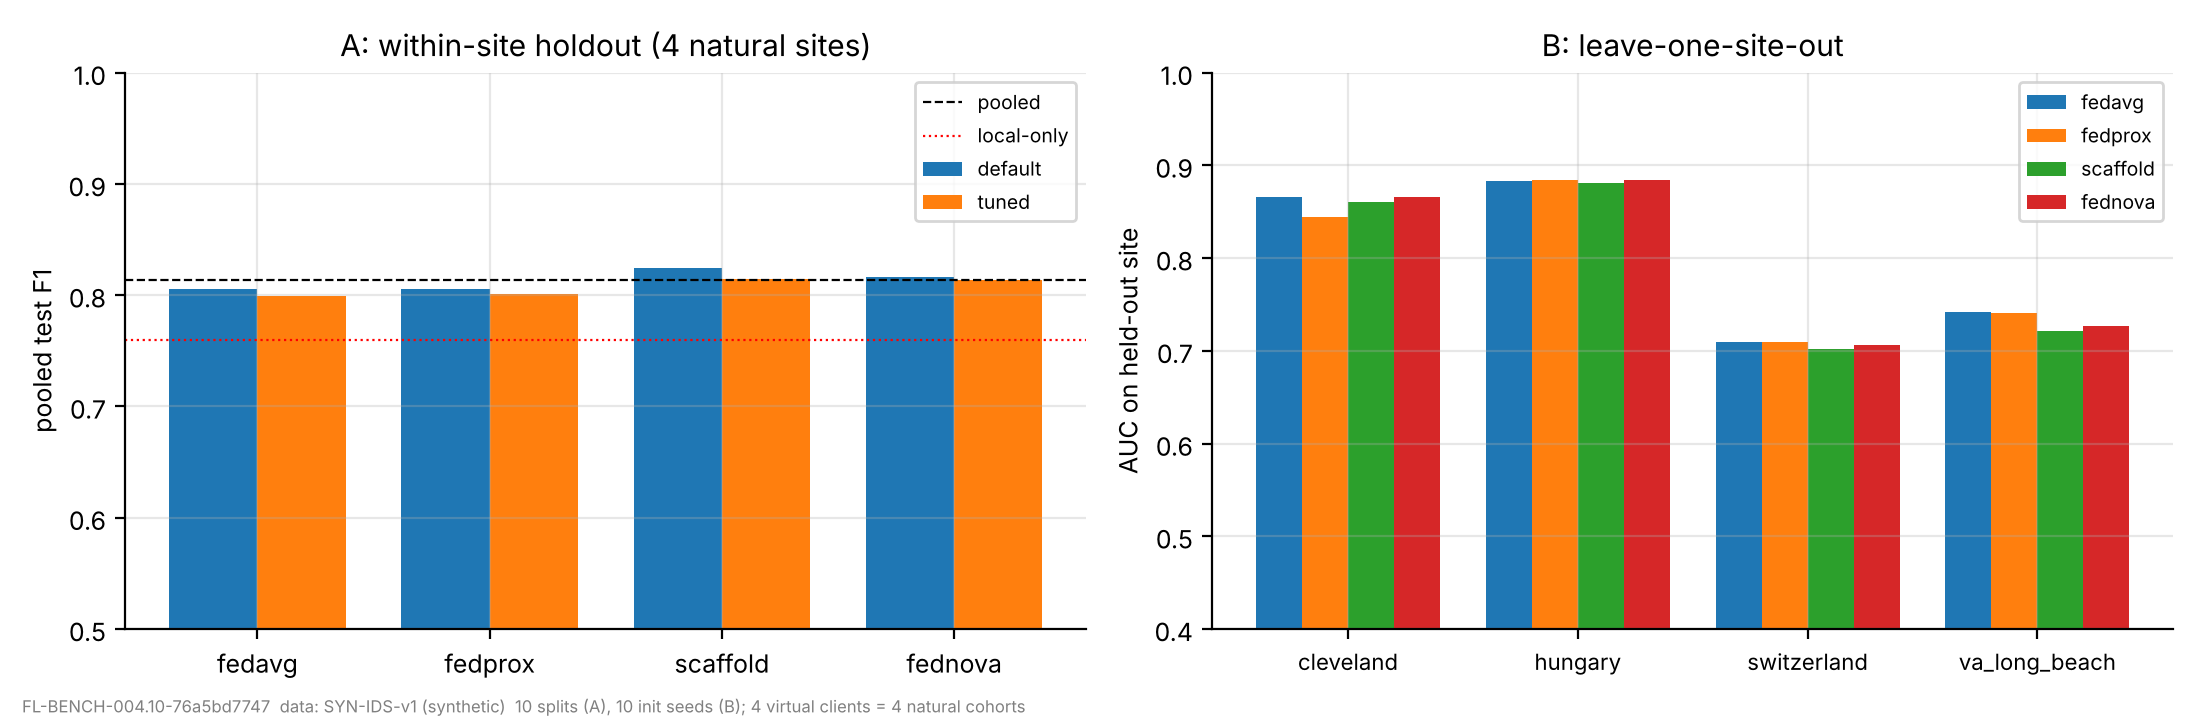
\includegraphics[width=0.95\textwidth]{figures/task_4_10_natural_sites.png}\caption{Natural-site benchmark. Left: pooled F1 (protocol A). Right: AUC on the held-out site (protocol B).}\label{f:sites}\end{figure*}
\subsubsection{Tuning more than the learning rate and $\mu$}
A 24-configuration random search over learning rate, $\mu$, batch size, local epochs, hidden width and SCAFFOLD server step changes test F1 relative to the lr/$\mu$ grid by between -0.011 (heart-4sites, FedAvg) and +0.018 (synthetic, FedNova) (Table~\ref{t:rs}); 1 of 8 paired random-vs-grid comparisons have uncorrected $p<0.05$. Budgets are matched in the number of configurations, not in compute, and selection on small validation sets can overfit. We therefore draw no conclusion about the best FL algorithm from this experiment.
\begin{table}[t]\centering\caption{Test F1: default, lr/$\mu$ grid, six-parameter random search.}\label{t:rs}\scriptsize
\begin{tabular}{lrrrr}\toprule
dataset & algo & default & grid & random \\\midrule
heart-4sites & fedavg & 0.808 & 0.807 & 0.796 \\
heart-4sites & fednova & 0.816 & 0.812 & 0.815 \\
heart-4sites & fedprox & 0.807 & 0.805 & 0.814 \\
heart-4sites & scaffold & 0.826 & 0.819 & 0.820 \\
synthetic & fedavg & 0.843 & 0.848 & 0.859 \\
synthetic & fednova & 0.864 & 0.855 & 0.873 \\
synthetic & fedprox & 0.839 & 0.858 & 0.855 \\
synthetic & scaffold & 0.873 & 0.801 & 0.814 \\\bottomrule\end{tabular}\end{table}
\subsection{Adaptive attackers (Q4)}\label{sec:adapt}
The tested defences are not robust to attackers that adapt (synthetic data, $K=20$, $f=4$). Against a static boosted backdoor the mean has ASR 1.00, while median, trimmed mean, Krum, Multi-Krum and the anomaly filter keep it low; adaptive variants raise it again for: anomaly\_filter (0.11$\to$0.65); krum (0.12$\to$1.00); multi\_krum (0.11$\to$0.76) (static$\to$adaptive ASR, Table~\ref{t:adb}). Untargeted ALIE and MIN-MAX alone barely moved accuracy in this setting (minimum accuracy 0.749 versus about 0.777 without attack).
\begin{table}[t]\centering\caption{Backdoor ASR, static vs adaptive attacks (synthetic).}\label{t:adb}\scriptsize
\resizebox{\columnwidth}{!}{\begin{tabular}{lrrrr}\toprule
defense & none\_clean & static\_boost & norm\_matched & minmax\_backdoor \\\midrule
anomaly\_filter & 0.107 & 0.106 & 0.498 & 0.649 \\
clip\_median\_norm & 0.111 & 0.788 & 0.775 & 0.639 \\
krum & 0.097 & 0.120 & 0.184 & 0.996 \\
mean & 0.106 & 0.998 & 0.753 & 0.636 \\
median & 0.113 & 0.261 & 0.257 & 0.266 \\
multi\_krum & 0.104 & 0.106 & 0.557 & 0.763 \\
trimmed\_mean & 0.114 & 0.288 & 0.290 & 0.311 \\\bottomrule\end{tabular}}\end{table}
Rule-aware attackers that simulate the server rule are stronger (Table~\ref{t:wc}): the worst-case accuracy drop per rule ranges from 0.016 to 0.411, the largest for mean under agr\_tailored; the AGR-aware backdoor reaches ASR above 0.5 on 5 of 7 rules (versus 5 for the distance-constrained backdoor). AGR-tailored was the strongest attack for 5 of 7 rules in the untargeted setting. Models destroyed outright (non-finite weights) are scored as constant predictors and counted; 6 of 630 untargeted runs ended with non-finite weights (all under AGR-tailored against the undefended mean).
\begin{table}[t]\centering\caption{Worst-case untargeted attack per aggregation rule (synthetic, $f=4$ of 20).}\label{t:wc}\scriptsize
\begin{tabular}{lrrrr}\toprule
defense & clean\_acc & worst\_attack & worst\_acc & drop \\\midrule
mean & 0.777 & agr\_tailored & 0.366 & 0.411 \\
median & 0.777 & fang & 0.756 & 0.020 \\
trimmed\_mean & 0.776 & fang & 0.755 & 0.020 \\
krum & 0.768 & agr\_tailored & 0.704 & 0.064 \\
multi\_krum & 0.775 & agr\_tailored & 0.753 & 0.022 \\
clip\_median\_norm & 0.774 & agr\_tailored & 0.744 & 0.031 \\
anomaly\_filter & 0.777 & agr\_tailored & 0.761 & 0.016 \\\bottomrule\end{tabular}\end{table}
\begin{figure*}[t]\centering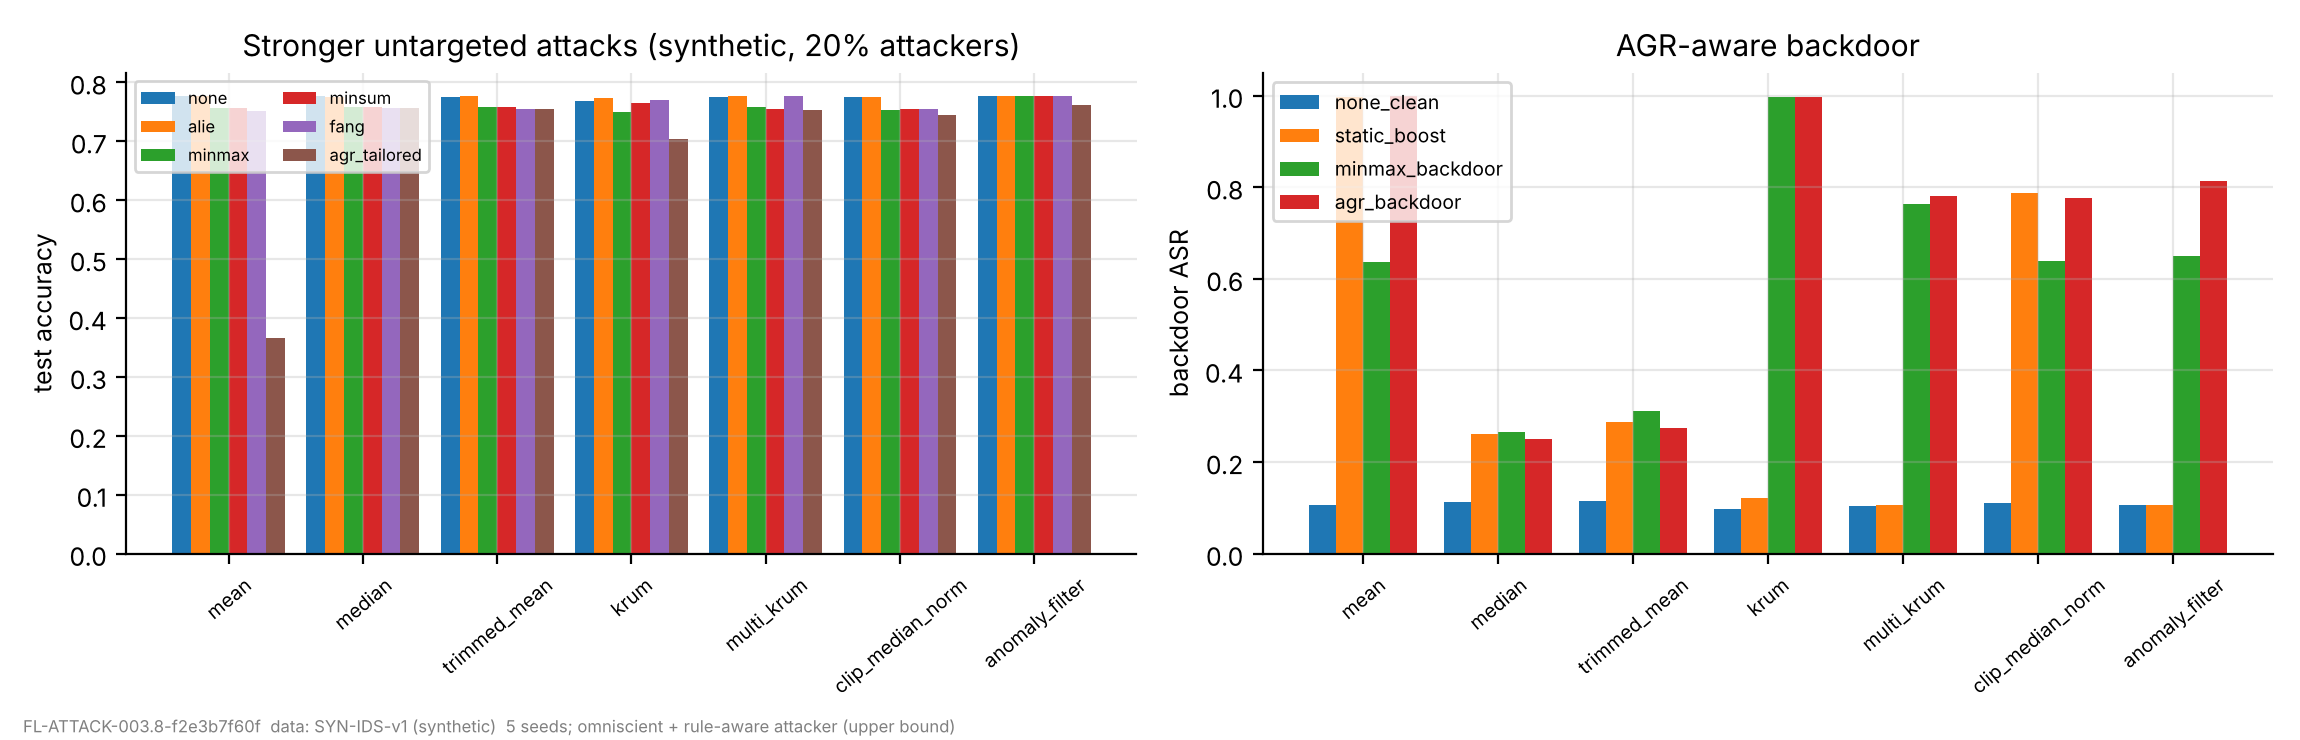
\includegraphics[width=0.95\textwidth]{figures/task_3_8_stronger_adaptive.png}\caption{Rule-aware adaptive attacks. Left: accuracy under untargeted attacks. Right: backdoor ASR.}\label{f:adapt}\end{figure*}
\subsection{Federated preprocessing and calibration}\label{sec:fp}
\subsubsection{Federated mean and variance}
The securely aggregated statistics match the pooled ones to within fixed-point precision: over 10 synthetic federations and 10 heart-disease splits the largest absolute deviation of any mean or standard deviation was 1.4e-10, and downstream F1 was identical to the pooled-mean oracle (mean difference +0.0000 on the heart sites). The price is two secure-aggregation rounds: 98\,KiB in total for 40 features and 10 clients (31\,ms in our process), and 13\,KiB for 10 features and 4 sites (Table~\ref{t:fp}). All three contrasts below use the pooled-mean oracle as reference, so imputation is matched across the compared arms; only the pooled-median row differs in imputation. Whether federated (global) standardisation is \emph{better} than local standardisation depends on the kind of heterogeneity. On SYN-TAB-40 with a per-client affine measurement shift that we injected ourselves, local standardisation removes the shift and wins by +0.114 F1 ($d_z=6.4$, Holm $p=0.006$ against the pooled mean). On the four natural heart-disease cohorts the order reverses: local standardisation loses 0.076 F1 ($d_z=-4.8$, Holm $p=0.008$). We have not isolated the cause. Plausible but untested reasons are that prevalence and missingness differ between the sites, so per-site standardisation also removes label-relevant signal, and that one site has very few negative cases. Replacing the pooled median by the global mean changed F1 by -0.0063 on the heart sites (Holm $p=0.016$, $d_z=-0.9$); the headline site results elsewhere in this paper still use the original pooled-median loader.
\begin{table}[t]\centering\caption{Effect of how features are standardised (FedAvg, 10 seeds or splits). $\Delta$F1 is the paired mean difference to the pooled-mean oracle; $d_z$ is the paired effect size.}\label{t:fp}\scriptsize
\resizebox{\columnwidth}{!}{\begin{tabular}{llrrr}\toprule
Data & Standardisation & F1 [95\% CI] & AUC & $\Delta$F1 vs pooled mean ($d_z$) \\\midrule
SYN-TAB-40, shifted clients & pooled mean (oracle) & 0.753 [0.740, 0.766] & 0.882 & -- \\
SYN-TAB-40, shifted clients & federated (secure sums) & 0.753 [0.740, 0.766] & 0.882 & +0.000 (0.1) \\
SYN-TAB-40, shifted clients & local only & 0.867 [0.861, 0.874] & 0.956 & +0.114 (6.4) \\
SYN-TAB-40, shifted clients & none & 0.787 [0.776, 0.798] & 0.905 & +0.034 (2.8) \\
heart, 4 sites & pooled median (original) & 0.806 [0.796, 0.816] & 0.859 & -0.006 (-0.9) \\
heart, 4 sites & pooled mean (oracle) & 0.812 [0.800, 0.824] & 0.861 & -- \\
heart, 4 sites & federated (secure sums) & 0.812 [0.800, 0.824] & 0.861 & +0.000 (0.0) \\
heart, 4 sites & local only & 0.736 [0.724, 0.749] & 0.799 & -0.076 (-4.8) \\
heart, 4 sites & none & 0.530 [0.327, 0.734] & 0.506 & -0.282 (-1.0) \\\bottomrule\end{tabular}}\end{table}
\subsubsection{Calibration}
Final-round calibration is moderate for all four algorithms: ECE lies between 0.032 and 0.077 and the Brier score between 0.075 and 0.151 (Table~\ref{t:cal}, 10 seeds). Against FedAvg, 1 of 12 Brier/ECE contrasts survive Holm correction within their family of three; the 95\% intervals of ECE share a common range on both data sets. The largest Brier difference is small in absolute terms (0.0094), so accuracy and F1 differences between the algorithms should not be read as calibration differences. On the heart data the test set holds roughly 280 rows, so ECE is noisy; we did not apply temperature scaling or any other recalibration, and a deployed risk model would need it validated on local data.
\begin{table}[t]\centering\caption{Calibration at the final round (10 seeds, no recalibration). Lower is better for both scores.}\label{t:cal}\scriptsize
\resizebox{\columnwidth}{!}{\begin{tabular}{llrrr}\toprule
Data & Algorithm & Brier [95\% CI] & ECE [95\% CI] & $\Delta$Brier vs FedAvg ($d_z$) \\\midrule
SYN-TAB-40, $\alpha=0.3$ & FedAvg & 0.085 [0.073, 0.096] & 0.045 [0.021, 0.070] & -- \\
SYN-TAB-40, $\alpha=0.3$ & FedProx & 0.086 [0.074, 0.098] & 0.044 [0.023, 0.065] & +0.0015 (0.8) \\
SYN-TAB-40, $\alpha=0.3$ & SCAFFOLD & 0.075 [0.067, 0.084] & 0.032 [0.020, 0.044] & -0.0094 (-0.6) \\
SYN-TAB-40, $\alpha=0.3$ & FedNova & 0.077 [0.070, 0.085] & 0.036 [0.021, 0.051] & -0.0074 (-0.7) \\
heart, 4 sites & FedAvg & 0.151 [0.144, 0.158] & 0.065 [0.055, 0.076] & -- \\
heart, 4 sites & FedProx & 0.151 [0.144, 0.158] & 0.065 [0.055, 0.075] & -0.0000 (-0.9) \\
heart, 4 sites & SCAFFOLD & 0.151 [0.144, 0.158] & 0.077 [0.061, 0.093] & -0.0003 (-0.1) \\
heart, 4 sites & FedNova & 0.150 [0.143, 0.157] & 0.073 [0.056, 0.090] & -0.0013 (-1.1) \\\bottomrule\end{tabular}}\end{table}
\begin{figure}[t]\centering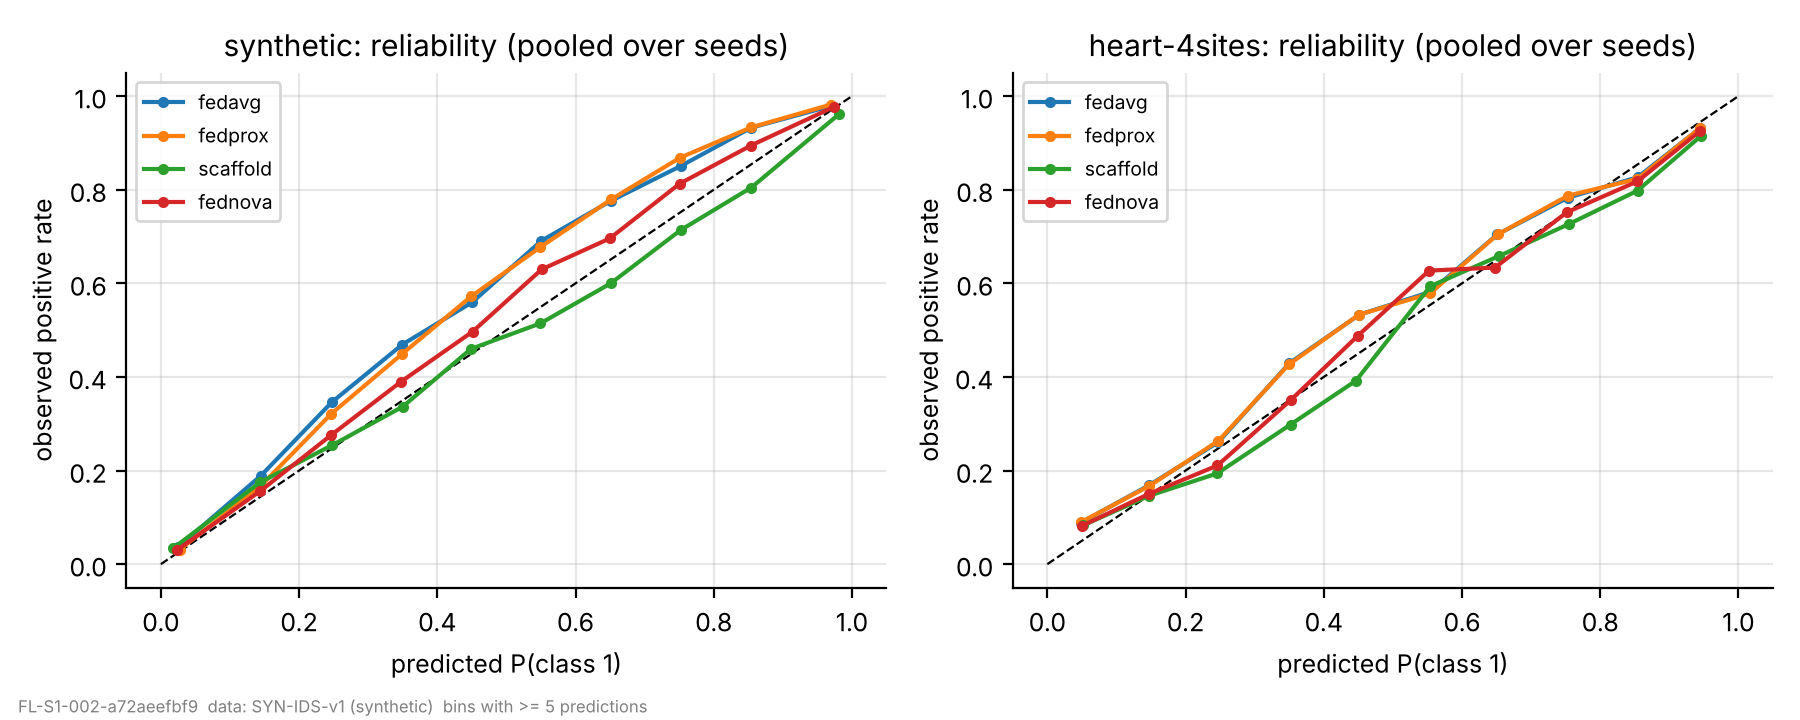
\includegraphics[width=\columnwidth]{figures/s1_2_reliability.png}\caption{Reliability diagrams pooled over seeds (bins with at least five predictions).}\label{f:rel}\end{figure}
\subsubsection{Sensitivity to malicious fraction, heterogeneity, participation and model size}
With sign-flip updates scaled by 5, the plain mean degrades from 0.775 accuracy without attackers to below 0.6 once 20\% of the clients are malicious (Table~\ref{t:mf}). Median and trimmed mean stay within 0.042 of their clean accuracy even at 40\% malicious clients; Krum is flat at about 0.768, which is 0.007 below the mean when nobody attacks. This is one attack behaviour against rules that suit it; the adaptive attackers of Section~\ref{sec:adapt} break the same rules. 16 of 18 aggregator-versus-mean contrasts are significant after Holm correction (10 seeds); from 10\% malicious clients on, the smallest paired effect size is $d_z=3.2$.
\begin{table}[t]\centering\caption{Test accuracy (mean$\pm$95\% half-width over 10 seeds) under sign-flip updates scaled by 5, $K=20$.}\label{t:mf}\scriptsize
\resizebox{\columnwidth}{!}{\begin{tabular}{lrrrr}\toprule
Malicious fraction & Mean & Median & Trimmed mean & Krum \\\midrule
0.00 & 0.775$\pm$0.007 & 0.774$\pm$0.008 & 0.775$\pm$0.007 & 0.768$\pm$0.007 \\
0.05 & 0.752$\pm$0.007 & 0.771$\pm$0.007 & 0.770$\pm$0.007 & 0.768$\pm$0.007 \\
0.10 & 0.711$\pm$0.010 & 0.768$\pm$0.007 & 0.767$\pm$0.007 & 0.768$\pm$0.008 \\
0.20 & 0.442$\pm$0.069 & 0.761$\pm$0.008 & 0.759$\pm$0.007 & 0.766$\pm$0.008 \\
0.30 & 0.432$\pm$0.066 & 0.753$\pm$0.006 & 0.751$\pm$0.006 & 0.768$\pm$0.007 \\
0.40 & 0.433$\pm$0.065 & 0.732$\pm$0.006 & 0.732$\pm$0.006 & 0.766$\pm$0.007 \\\bottomrule\end{tabular}}\end{table}
Label skew matters more than the choice of algorithm (Table~\ref{t:al}). Between $\alpha=1$ and $\alpha=0.1$ FedAvg loses 0.107 accuracy, while the largest gain of any other strategy over FedAvg at a given $\alpha$ is +0.031 (scaffold, $\alpha=0.1$, $d_z=0.3$). Robust aggregation has a price that grows with heterogeneity even without any attacker: the coordinate median costs 0.042 accuracy at $\alpha=1$ and 0.175 at $\alpha=0.1$, because honest but dissimilar clients look like outliers. 11 of 20 strategy-or-robust-rule-versus-FedAvg contrasts are significant after Holm correction.
\begin{table}[t]\centering\caption{Test accuracy (mean$\pm$95\% half-width over 10 seeds) by Dirichlet concentration $\alpha$ (smaller = more skew), clean data, $K=10$.}\label{t:al}\scriptsize
\resizebox{\columnwidth}{!}{\begin{tabular}{lrrrrrr}\toprule
$\alpha$ & FedAvg & FedProx & SCAFFOLD & FedNova & FedAvg+median & FedAvg+trimmed \\\midrule
0.1 & 0.782$\pm$0.051 & 0.780$\pm$0.046 & 0.813$\pm$0.112 & 0.811$\pm$0.024 & 0.607$\pm$0.086 & 0.702$\pm$0.086 \\
0.3 & 0.865$\pm$0.028 & 0.860$\pm$0.027 & 0.886$\pm$0.022 & 0.882$\pm$0.017 & 0.749$\pm$0.043 & 0.802$\pm$0.027 \\
0.5 & 0.881$\pm$0.014 & 0.876$\pm$0.015 & 0.899$\pm$0.004 & 0.887$\pm$0.012 & 0.816$\pm$0.024 & 0.842$\pm$0.015 \\
1 & 0.889$\pm$0.009 & 0.884$\pm$0.010 & 0.901$\pm$0.004 & 0.890$\pm$0.008 & 0.846$\pm$0.032 & 0.870$\pm$0.011 \\\bottomrule\end{tabular}}\end{table}
Participation matters for robust rules because the number of clients in a round shrinks. At a 10\% participation rate only two of 20 clients train per round, and the coordinate median of two updates is simply their mean: with 20\% sign-flip clients accuracy falls to 0.545 (clean mean at the same rate: 0.773); at full participation the median holds 0.761. Model size changes accuracy modestly (0.757 at 346 parameters, 0.794 at 5506) while per-experiment communication grows linearly from 1.1 to 16.8\,MB. All four grids use $K\le 20$ virtual clients on synthetic data, so they show the direction and rough size of effects, not rates for real deployments.
\begin{figure*}[t]\centering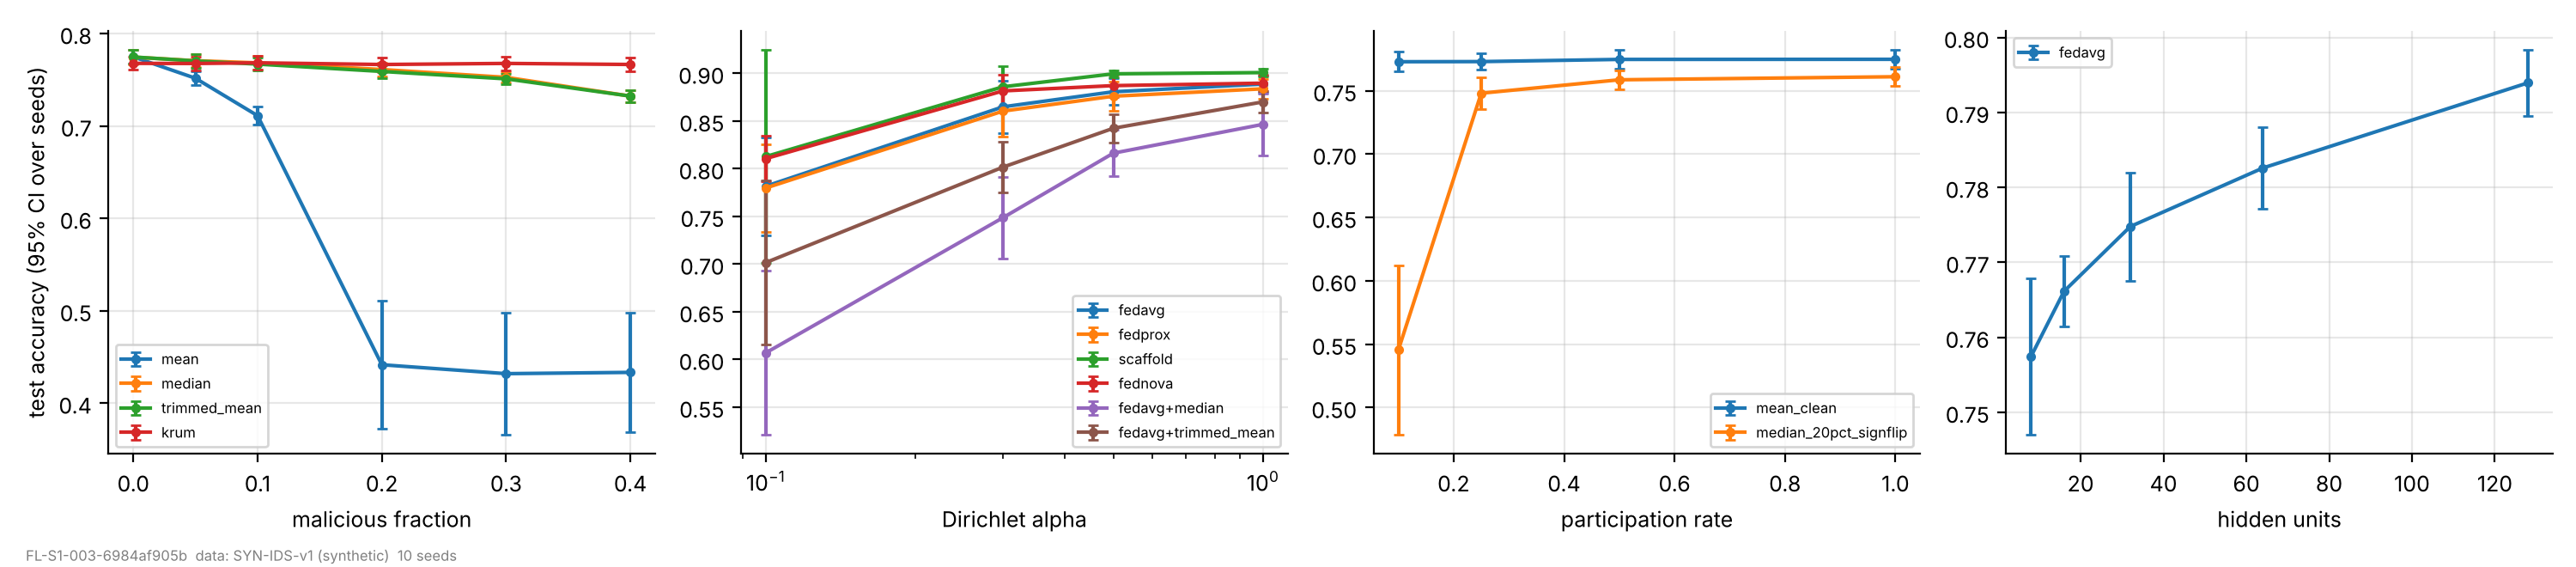
\includegraphics[width=0.95\textwidth]{figures/s1_3_ablation_grids.png}\caption{One-factor sensitivity grids (10 seeds; bars are 95\% $t$-intervals).}\label{f:s13}\end{figure*}
\subsection{Literature defences and model baselines}\label{sec:lit}
\subsubsection{Untargeted attacks}
Table~\ref{t:s2u} puts the four new rules next to the seven earlier ones under the same attacks (10 seeds). Judged by the worst accuracy over the five scenarios, the best earlier rule is anomaly filter (0.758) and the best of the new rules is FLAME ($\lambda{=}0.001$) (0.754); the mean falls to 0.384. Without any attacker the new rules cost between +0.003 and +0.010 accuracy relative to the plain mean. Against the rule-simulating attacker FLAME ($\lambda{=}0$), FLAME ($\lambda{=}0.001$), SignGuard stay within 0.02 of the median (0.755: FLAME ($\lambda{=}0$) 0.754, FLAME ($\lambda{=}0.001$) 0.754, SignGuard 0.738); RLR (0.407) collapses towards the mean (0.384), and the FoolsGold cell for this attacker is withdrawn (Section~\ref{sec:fgdefect}); under plain sign flipping the new rules score FLAME ($\lambda{=}0$) 0.773, FLAME ($\lambda{=}0.001$) 0.773, RLR 0.432, FoolsGold 0.434, SignGuard 0.773 (median 0.761, mean 0.442). RLR and FoolsGold were designed for other threats (backdoors; sybils with similar updates) and are not expected to stop independent Byzantine updates, which is what we see for both under sign flipping and for RLR under the rule-simulating attacker. Of 35 paired contrasts of a new rule against the mean (five scenarios, i.i.d.\ and skewed), 8 show a significantly higher accuracy for the new rule after Holm correction. Each correction is applied within its own scenario, so 8 of 35 is a count of tests and not a family-wise result over all 35. Three of the 35 contrasts are FoolsGold under ALIE, MIN-MAX and the AGR-tailored attacker, whose cells are affected by the defect described in Section~\ref{sec:fgdefect}; none is among the 8, and recomputing the Holm correction within those three scenarios without FoolsGold leaves the eight unchanged. All of this holds for one synthetic data set, one attacker fraction (20\%) and an omniscient attacker, which is an upper bound; the numbers describe these rules in this setting, not their general quality.
\begin{table}[t]\centering\caption{Test accuracy (mean$\pm$95\% half-width over 10 seeds), $K=20$, $f=4$ colluding attackers, i.i.d.\ clients. New rules are those re-implemented in this stage. $^\dagger$ Withdrawn: the AGR-tailored attacker triggered a defect in our FoolsGold implementation (Section~\ref{sec:fgdefect}). $^\ddagger$ Computed with the defective implementation (Section~\ref{sec:fgdefect}); kept for the record, not repaired.}\label{t:s2u}\scriptsize
\resizebox{\columnwidth}{!}{\begin{tabular}{lrrrrr}\toprule
Rule & no attack & sign flip & ALIE & MIN-MAX & AGR-tailored \\\midrule
mean & 0.775$\pm$0.007 & 0.442$\pm$0.069 & 0.775$\pm$0.007 & 0.755$\pm$0.006 & 0.384$\pm$0.027 \\
median & 0.774$\pm$0.008 & 0.761$\pm$0.008 & 0.773$\pm$0.008 & 0.756$\pm$0.006 & 0.755$\pm$0.006 \\
trimmed mean & 0.774$\pm$0.008 & 0.759$\pm$0.007 & 0.774$\pm$0.008 & 0.756$\pm$0.006 & 0.754$\pm$0.006 \\
Krum & 0.767$\pm$0.007 & 0.766$\pm$0.008 & 0.772$\pm$0.008 & 0.750$\pm$0.012 & 0.700$\pm$0.013 \\
Multi-Krum & 0.773$\pm$0.007 & 0.775$\pm$0.007 & 0.774$\pm$0.008 & 0.756$\pm$0.005 & 0.752$\pm$0.005 \\
median-norm clip & 0.772$\pm$0.007 & 0.748$\pm$0.004 & 0.772$\pm$0.008 & 0.753$\pm$0.005 & 0.743$\pm$0.005 \\
anomaly filter & 0.775$\pm$0.007 & 0.775$\pm$0.007 & 0.775$\pm$0.007 & 0.775$\pm$0.007 & 0.758$\pm$0.006 \\
FLAME ($\lambda{=}0$) (new) & 0.772$\pm$0.008 & 0.773$\pm$0.008 & 0.772$\pm$0.009 & 0.770$\pm$0.008 & 0.754$\pm$0.005 \\
FLAME ($\lambda{=}0.001$) (new) & 0.772$\pm$0.007 & 0.773$\pm$0.008 & 0.773$\pm$0.009 & 0.771$\pm$0.008 & 0.754$\pm$0.005 \\
RLR (new) & 0.764$\pm$0.007 & 0.432$\pm$0.044 & 0.769$\pm$0.008 & 0.729$\pm$0.008 & 0.407$\pm$0.027 \\
FoolsGold (new) & 0.764$\pm$0.013 & 0.434$\pm$0.064 & 0.763$\pm$0.008$^\ddagger$ & 0.748$\pm$0.012$^\ddagger$ & --$^\dagger$ \\
SignGuard (new) & 0.772$\pm$0.008 & 0.773$\pm$0.007 & 0.771$\pm$0.007 & 0.753$\pm$0.006 & 0.738$\pm$0.006 \\\bottomrule\end{tabular}}\end{table}
\subsubsection{A defect in our FoolsGold implementation}\label{sec:fgdefect}
After this stage was run we found that our FoolsGold implementation gives full weight to clients whose accumulated update histories have cosine similarity exactly 1: the logit rescaling then evaluates $\ln 0=-\infty$, and the code replaces non-finite values by 1 instead of 0. Colluders that submit bit-identical updates therefore escape the defence. In a one-seed check (i.i.d., seed 0, 20 rounds) the update chosen by the AGR-tailored attacker triggered this in 20 of 20 rounds (on average 61\% of the 34 candidates it considers do). ALIE and MIN-MAX trigger it in some rounds. Sign flipping did not trigger it in the rounds we checked, and the static, norm-matched and AGR-backdoor attackers did not trigger it in Table~\ref{t:s2d} (rejection 1.00); we did not check the backdoor tables of the later stages for it separately. The AGR-tailored FoolsGold cells are therefore withdrawn and the ALIE and MIN-MAX cells are marked in Tables~\ref{t:s2u} and~\ref{t:s2d}. We did not repeat the affected runs. A corrected variant (\texttt{allfeat\_corrected}) is included in the accompanying archive but was not used for the results above.
\subsubsection{Backdoor attacks}
The picture for backdoors differs by rule (Table~\ref{t:s2b}, 10 seeds; ASR is the share of triggered test samples classified as the target class). FoolsGold keeps the ASR at or below 0.178 in every scenario, including the AGR-backdoor attacker, and rejects the colluding clients almost always (TPR 1.00, FPR 0.03). That is the setting it was designed for: our four attackers train on the same kind of poisoned data and their updates are therefore similar, and our adaptive attackers do not try to decorrelate their updates. We did not test an attacker that optimises its decorrelation against the rule. The only diversification we did test is the random jitter of Table~\ref{t:s3b} (5 seeds, exploratory), which raises FoolsGold's ASR from 0.512 to 0.804 with wide, overlapping intervals; this result should therefore not be read as robustness to sybils that diversify. FLAME stops the static and norm-matched backdoors (ASR 0.117 and 0.237) but not the AGR-backdoor attacker (0.844); RLR with our $\theta$ does not stop the boosted backdoors on i.i.d.\ clients (0.989); SignGuard stops the static boost (0.114) but not the norm-matched or AGR-backdoor attackers (0.715, 0.849). Rules with a worst-case ASR below 0.3 over the three attacks: median, trimmed mean, FoolsGold.
\begin{table}[t]\centering\caption{Backdoor attack success rate (mean$\pm$95\% half-width over 10 seeds; 20 rounds, 12\,000 samples), $K=20$, $f=4$, i.i.d.\ clients. Without attackers the plain mean has ASR 0.114. The no-attack column is the floor, so compare rules by the excess over it (FoolsGold under the AGR-backdoor attacker: $+0.030$); levels are not comparable with Table~\ref{t:s3b} (15 rounds, 8\,000 samples).}\label{t:s2b}\scriptsize
\resizebox{\columnwidth}{!}{\begin{tabular}{lrrrr}\toprule
Rule & no attack & static boost & norm-matched & AGR-backdoor \\\midrule
mean & 0.114$\pm$0.062 & 0.998$\pm$0.001 & 0.720$\pm$0.100 & 1.000$\pm$0.000 \\
median & 0.115$\pm$0.063 & 0.245$\pm$0.118 & 0.252$\pm$0.112 & 0.242$\pm$0.116 \\
trimmed mean & 0.117$\pm$0.064 & 0.273$\pm$0.125 & 0.283$\pm$0.119 & 0.266$\pm$0.122 \\
Krum & 0.120$\pm$0.069 & 0.129$\pm$0.067 & 0.242$\pm$0.171 & 0.994$\pm$0.003 \\
Multi-Krum & 0.114$\pm$0.062 & 0.112$\pm$0.057 & 0.539$\pm$0.139 & 0.747$\pm$0.093 \\
median-norm clip & 0.117$\pm$0.062 & 0.755$\pm$0.091 & 0.741$\pm$0.094 & 0.742$\pm$0.093 \\
anomaly filter & 0.114$\pm$0.061 & 0.112$\pm$0.057 & 0.471$\pm$0.146 & 0.772$\pm$0.102 \\
FLAME ($\lambda{=}0$) (new) & 0.120$\pm$0.064 & 0.117$\pm$0.057 & 0.237$\pm$0.131 & 0.844$\pm$0.069 \\
FLAME ($\lambda{=}0.001$) (new) & 0.121$\pm$0.063 & 0.117$\pm$0.057 & 0.237$\pm$0.134 & 0.848$\pm$0.068 \\
RLR (new) & 0.179$\pm$0.085 & 0.989$\pm$0.005 & 0.190$\pm$0.098 & 1.000$\pm$0.000 \\
FoolsGold (new) & 0.148$\pm$0.085 & 0.178$\pm$0.114 & 0.178$\pm$0.114 & 0.178$\pm$0.115 \\
SignGuard (new) & 0.116$\pm$0.063 & 0.114$\pm$0.057 & 0.715$\pm$0.131 & 0.849$\pm$0.072 \\\bottomrule\end{tabular}}\end{table}
Detection rates explain part of this (Table~\ref{t:s2d}). FLAME rejects on average 43\% of the honest rows per round under attack; we did not isolate the cause, a plausible one being the minimum-cluster-size rule when honest updates are spread out. SignGuard's FPR is 0.19 on average; its TPR is 1.00 against ALIE but 0.01 against the AGR-tailored attacker and 0.07 against the AGR-backdoor attacker. A rate is an average over rounds and clients; it does not tell which rounds were fatal.
\begin{table}[t]\centering\caption{Share of malicious rows rejected / share of honest rows rejected (TPR/FPR, mean over rounds and 10--10 seeds), i.i.d.\ clients, $f=4$ of 20. Untargeted attacks first, then backdoors. $^\dagger$ and $^\ddagger$ as in Table~\ref{t:s2u}.}\label{t:s2d}\scriptsize
\resizebox{\columnwidth}{!}{\begin{tabular}{lrrrrrrr}\toprule
Rule & sign flip & ALIE & MIN-MAX & AGR-tail. & static & norm-m. & AGR-bd \\\midrule
anomaly filter & 1.00/0.00 & 0.06/0.00 & 0.98/0.01 & 0.00/0.01 & 1.00/0.00 & 0.41/0.06 & 0.03/0.01 \\
Multi-Krum & 1.00/0.00 & 0.00/0.25 & 0.24/0.19 & 0.00/0.25 & 1.00/0.00 & 0.55/0.11 & 0.00/0.25 \\
FLAME ($\lambda{=}0$) & 1.00/0.30 & 0.00/0.56 & 0.94/0.31 & 0.00/0.53 & 1.00/0.30 & 0.91/0.31 & 0.00/0.52 \\
FoolsGold & 0.05/0.04 & 0.35/0.02$^\ddagger$ & 0.34/0.03$^\ddagger$ & --$^\dagger$ & 1.00/0.03 & 1.00/0.03 & 1.00/0.03 \\
SignGuard & 1.00/0.17 & 1.00/0.01 & 0.35/0.28 & 0.01/0.32 & 1.00/0.22 & 0.22/0.20 & 0.07/0.27 \\\bottomrule\end{tabular}}\end{table}
Label skew changes the ranking (Table~\ref{t:s2n}). With Dirichlet $\alpha=0.3$ and no attacker, 10 of the 11 other rules lose accuracy against the mean (0.799); the largest loss is 0.249 (FLAME ($\lambda{=}0.001$)). Under the static boosted backdoor on skewed clients the ASR of FLAME is 0.459, of RLR 0.314 and of FoolsGold 0.551, but their clean accuracy is 0.635, 0.686 and 0.607. A defence that lowers the ASR by lowering accuracy for everyone is not a good trade, so the two numbers must be read together.
\begin{table}[t]\centering\caption{Cost of each rule under label skew (Dirichlet $\alpha=0.3$) (10--10 seeds; i.i.d.\ column for comparison).}\label{t:s2n}\scriptsize
\resizebox{\columnwidth}{!}{\begin{tabular}{lrrrr}\toprule
Rule & acc, i.i.d., none & acc, skew, none & acc, skew, sign flip & ASR, skew, static \\\midrule
mean & 0.775 & 0.799 & 0.519 & 0.995 \\
median & 0.774 & 0.686 & 0.553 & 0.812 \\
trimmed mean & 0.774 & 0.705 & 0.600 & 0.804 \\
Krum & 0.767 & 0.578 & 0.526 & 0.626 \\
Multi-Krum & 0.773 & 0.681 & 0.663 & 0.728 \\
median-norm clip & 0.772 & 0.745 & 0.613 & 0.951 \\
anomaly filter & 0.775 & 0.805 & 0.678 & 0.775 \\
FLAME ($\lambda{=}0$) (new) & 0.772 & 0.551 & 0.594 & 0.459 \\
FLAME ($\lambda{=}0.001$) (new) & 0.772 & 0.550 & 0.593 & 0.458 \\
RLR (new) & 0.764 & 0.647 & 0.553 & 0.314 \\
FoolsGold (new) & 0.764 & 0.623 & 0.524 & 0.551 \\
SignGuard (new) & 0.772 & 0.655 & 0.609 & 0.731 \\\bottomrule\end{tabular}}\end{table}
\begin{figure*}[t]\centering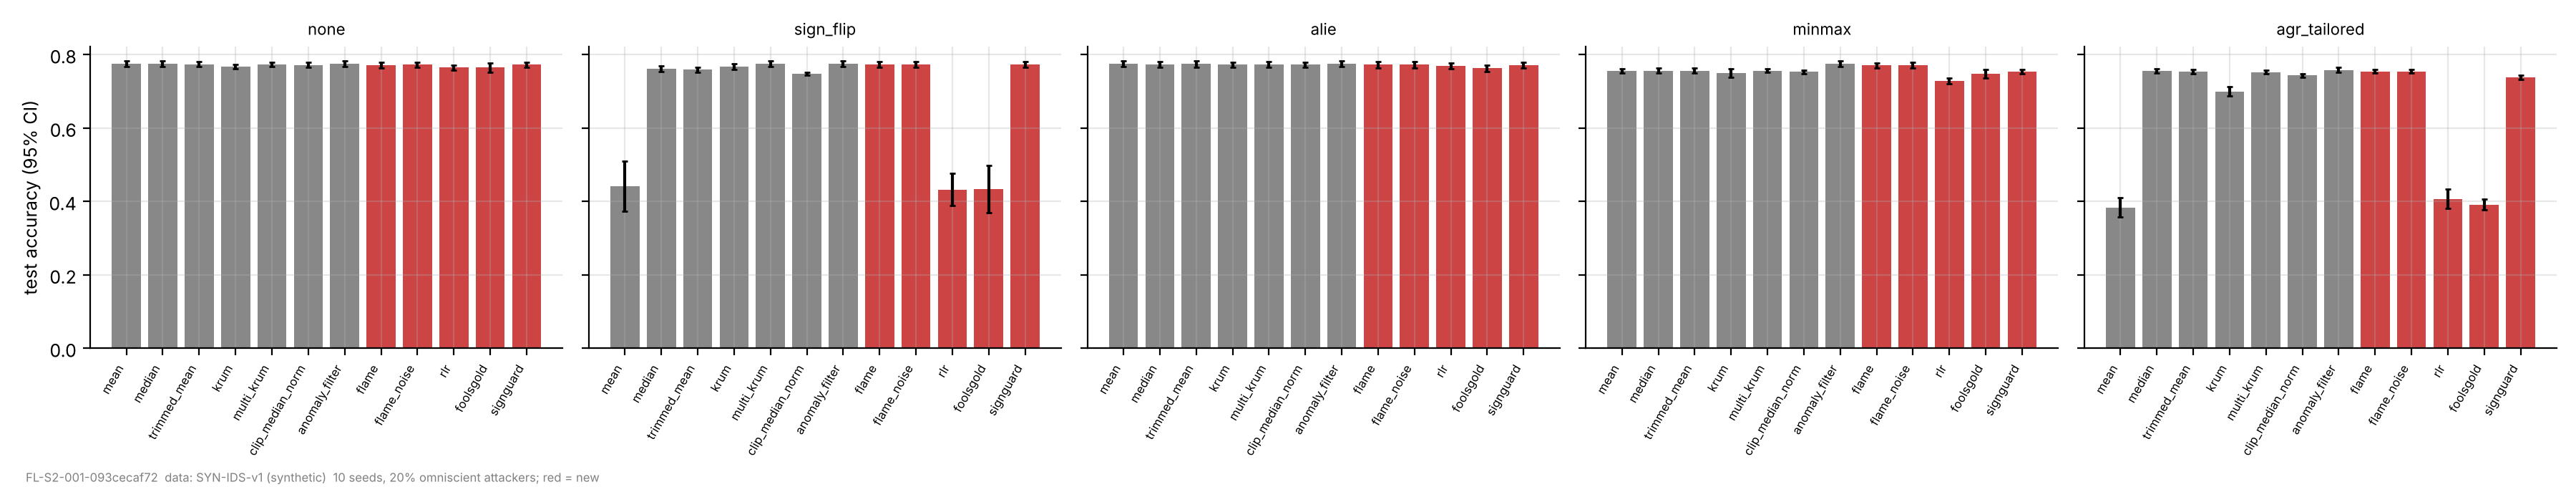
\includegraphics[width=0.95\textwidth]{figures/s2_1_untargeted.png}\caption{Accuracy of twelve rules under five untargeted scenarios (red: new rules; 95\% $t$-intervals over seeds).}\label{f:s2u}\end{figure*}
\begin{figure*}[t]\centering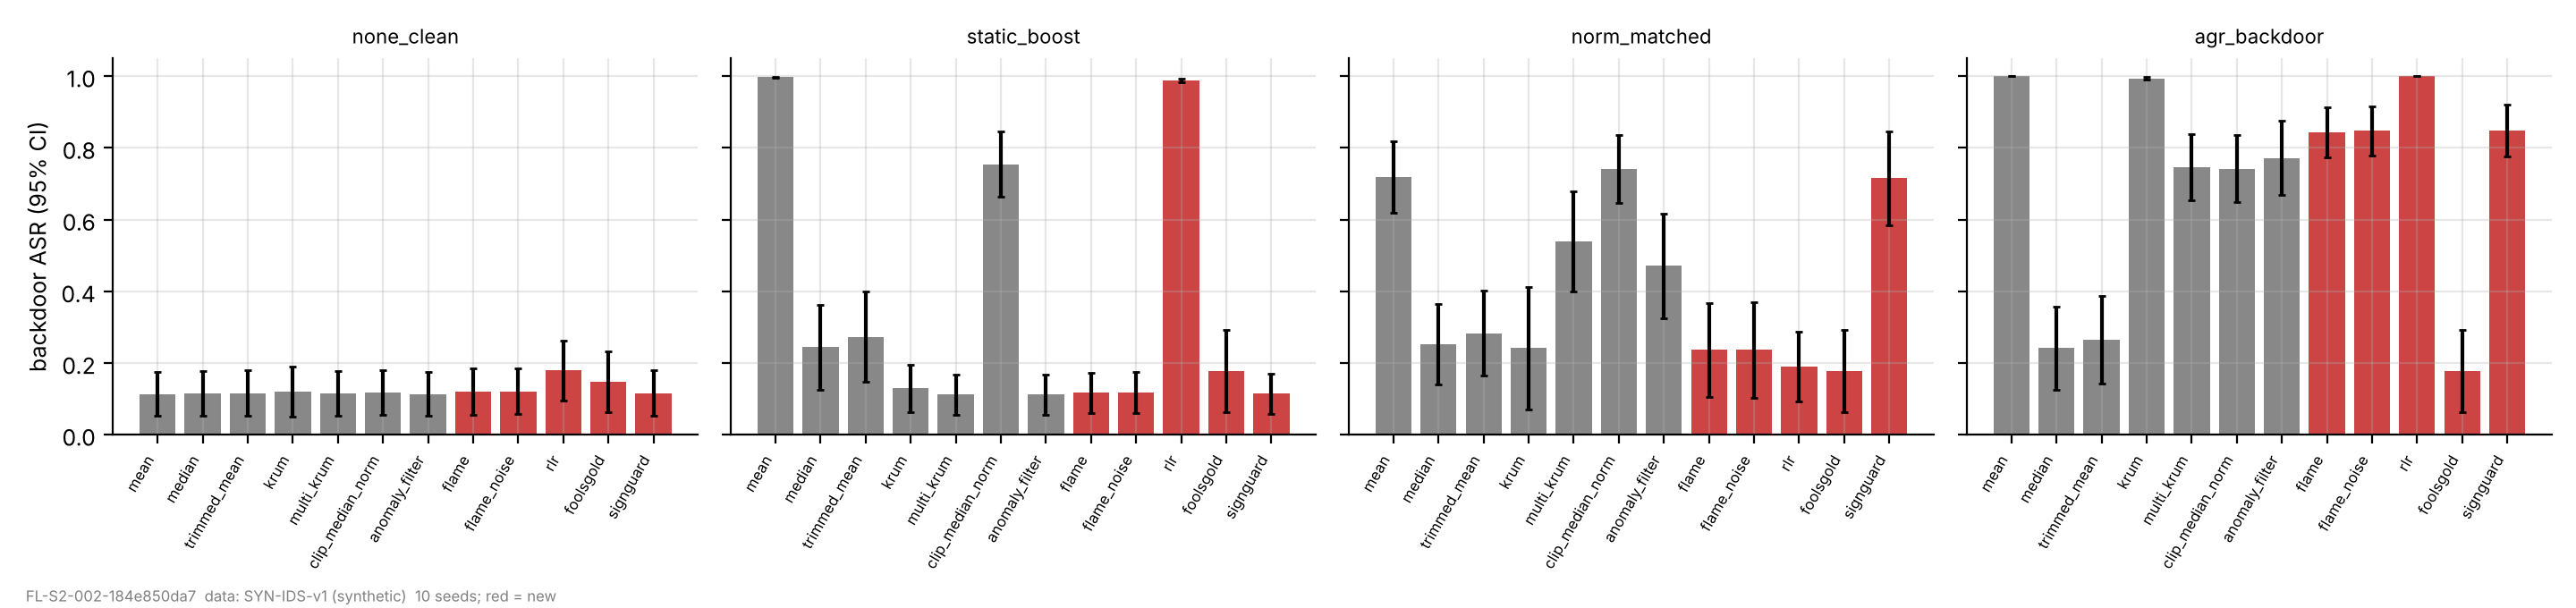
\includegraphics[width=0.95\textwidth]{figures/s2_2_backdoor.png}\caption{Backdoor ASR of twelve rules (red: new rules; 95\% $t$-intervals over seeds).}\label{f:s2b}\end{figure*}
\subsubsection{Model baselines}
A linear model is a strong test of whether the MLP is needed. Under FedAvg on SYN-TAB-40 logistic regression reaches F1 0.553, the one-hidden-layer MLP 0.859 and the three-hidden-layer MLP 0.858 (Table~\ref{t:s2a}, 10 seeds, same learning rate, rounds and local epochs for all three, no per-model tuning). On the four heart-disease cohorts the corresponding values are 0.803, 0.803 and 0.805. Under 20\% sign-flip clients the plain mean gives accuracy 0.396 (logistic regression), 0.442 (MLP) and 0.461 (deep MLP), and the median 0.723, 0.761 and 0.629 (the deep MLP's F1 under the median is 0.154, which suggests it mostly predicts one class). The gaps therefore describe this synthetic generator, which has nonlinear structure by construction, and small cohorts. They should not be transferred to other data.
\begin{table}[t]\centering\caption{Model baselines (10 seeds or splits). FedAvg: $K=10$ clients (Dirichlet $\alpha=0.3$) on SYN-TAB-40, the four natural sites on the heart data; pooled SGD uses the same total number of local passes.}\label{t:s2a}\scriptsize
\resizebox{\columnwidth}{!}{\begin{tabular}{lllrrr}\toprule
Data & Training & Model & F1 [95\% CI] & AUC & $\Delta$F1 vs MLP ($d_z$) \\\midrule
SYN-TAB-40 & FedAvg & logistic regression & 0.553 [0.499, 0.606] & 0.783 & -0.306 (-5.2) \\
SYN-TAB-40 & FedAvg & MLP (1 hidden) & 0.859 [0.842, 0.876] & 0.959 & -- \\
SYN-TAB-40 & FedAvg & MLP (3 hidden) & 0.858 [0.843, 0.874] & 0.955 & -0.001 (-0.1) \\
SYN-TAB-40 & pooled SGD & logistic regression & 0.621 [0.613, 0.628] & 0.778 & -0.267 (-30.9) \\
SYN-TAB-40 & pooled SGD & MLP (1 hidden) & 0.887 [0.882, 0.892] & 0.965 & -- \\
SYN-TAB-40 & pooled SGD & MLP (3 hidden) & 0.905 [0.899, 0.911] & 0.968 & +0.018 (2.4) \\
heart, 4 sites & FedAvg & logistic regression & 0.803 [0.790, 0.816] & 0.858 & -0.000 (-0.0) \\
heart, 4 sites & FedAvg & MLP (1 hidden) & 0.803 [0.791, 0.816] & 0.857 & -- \\
heart, 4 sites & FedAvg & MLP (3 hidden) & 0.805 [0.792, 0.818] & 0.850 & +0.002 (0.1) \\
heart, 4 sites & pooled SGD & logistic regression & 0.813 [0.799, 0.826] & 0.857 & +0.012 (0.4) \\
heart, 4 sites & pooled SGD & MLP (1 hidden) & 0.801 [0.781, 0.821] & 0.840 & -- \\
heart, 4 sites & pooled SGD & MLP (3 hidden) & 0.758 [0.689, 0.827] & 0.815 & -0.043 (-0.6) \\\bottomrule\end{tabular}}\end{table}
\subsection{Rule committee under the knowledge ladder (exploratory)}\label{sec:s3}
This section is exploratory. It uses 5 seeds for the untargeted and 5 for the backdoor comparison (the twelve-rule comparison above used 10), and the differences between rules are small compared with the interval half-widths, which overlap across almost all conditions. The main finding is therefore a null result, which rests on the effect sizes and the interval overlap and not on a significance test: the committee did not beat its best member or the median, and we found no measurable benefit of randomisation. The point estimates follow.
Table~\ref{t:s3u} reports accuracy (5 seeds). Against the draw-aware AGR-tailored attacker the best committee variant (committee, all 4, vote$\ge$2) reaches 0.725, the best single member (anomaly filter) 0.715, the worst single member 0.675 and the coordinate-wise median 0.718; the plain mean reaches 0.394. The differences among median, members and committees are small compared with the interval half-widths, and none of 140 paired contrasts (against the median and FoolsGold) is significant after Holm correction, but this carries no evidential weight: with 5 seeds the smallest possible exact two-sided Wilcoxon $p$-value is 0.0625, and Holm correction over 140 contrasts requires $p<0.00036$, so no contrast could have reached significance. We therefore rely on the effect sizes ($d_z$ and Cliff's $\delta$) in the stored test file. Lowering the attacker's knowledge from draw-aware to pool-aware changed the accuracy of the two random committees by +0.014 and +0.009, which is within the interval widths in this data; we therefore \emph{cannot} claim that randomisation measurably helped here. Under label skew (Dirichlet $\alpha{=}0.3$, no attacker) the committees lose between 0.156 and 0.189 accuracy relative to the mean, against 0.028 to 0.142 for single members, and under attack with skew the best single member (anomaly filter, 0.626) is ahead of every committee (0.562 at best).
\begin{table}[t]\centering\caption{Test accuracy (mean$\pm$95\% half-width over 5 seeds), $K=20$, $f=4$ colluding omniscient attackers, i.i.d.\ clients. ``pool'' rows: attacker does not know the random draw; only randomised committees are listed there (for deterministic rules the two knowledge levels coincide).}\label{t:s3u}\scriptsize
\resizebox{\columnwidth}{!}{\begin{tabular}{lrrrrr}\toprule
Rule & none & AGR & AGR, pool & AGR+jitter & AGR+jitter, pool \\\midrule
median & 0.745$\pm$0.010 & 0.718$\pm$0.012 & -- & 0.726$\pm$0.014 & -- \\
Multi-Krum & 0.744$\pm$0.010 & 0.715$\pm$0.009 & -- & 0.717$\pm$0.008 & -- \\
FLAME & 0.742$\pm$0.011 & 0.711$\pm$0.015 & -- & 0.712$\pm$0.015 & -- \\
SignGuard & 0.739$\pm$0.009 & 0.675$\pm$0.026 & -- & 0.718$\pm$0.016 & -- \\
anomaly filter & 0.743$\pm$0.008 & 0.715$\pm$0.009 & -- & 0.737$\pm$0.013 & -- \\
committee, all 4, vote$\ge$1 & 0.743$\pm$0.011 & 0.718$\pm$0.013 & -- & 0.736$\pm$0.011 & -- \\
committee, all 4, vote$\ge$2 & 0.742$\pm$0.011 & 0.725$\pm$0.012 & -- & 0.730$\pm$0.012 & -- \\
random committee, $k{=}2$, vote$\ge$1 & 0.742$\pm$0.011 & 0.716$\pm$0.013 & 0.729$\pm$0.015 & 0.725$\pm$0.013 & 0.734$\pm$0.011 \\
random committee, $k{=}3$, vote$\ge$2 & 0.742$\pm$0.011 & 0.716$\pm$0.012 & 0.725$\pm$0.014 & 0.724$\pm$0.011 & 0.731$\pm$0.015 \\\bottomrule\end{tabular}}\end{table}
For the backdoor (Table~\ref{t:s3b}, 5 seeds; ASR without any attacker is 0.387 for the median) the idealised AGR-backdoor attacker with identical malicious rows gets ASR 0.543 against the median and 0.512 against FoolsGold, but 0.840 to 0.892 against the committees: so the point estimates favour the median on this attack. The ASR intervals are very wide (the seed-to-seed spread of the backdoor outcome is large, and the no-attack ASR is already about 0.4 because the target class is common), so the intervals of median and committees overlap and this ordering is suggestive only. Once the colluders' rows are jittered, Multi-Krum alone gives ASR 0.384 and the committees 0.400--0.414, i.e.\ the committee matches but does not improve on its best member, while FoolsGold, which relies on similar updates, degrades to 0.804. With the caveat that the intervals overlap, a pool-aware attacker obtains 0.787 and 0.822 against the two random committees, compared with 0.876 and 0.840 for a draw-aware one.
\begin{table}[t]\centering\caption{Backdoor attack success rate (mean$\pm$95\% half-width over 5 seeds; 15 rounds, 8\,000 samples), $K=20$, $f=4$, i.i.d.\ clients. The no-attack column is the floor (about 0.4, because the target class is common), so compare rules by the excess over it (FoolsGold: $+0.079$ for AGR-bd, $+0.371$ with jitter); levels are not comparable with Table~\ref{t:s2b} (20 rounds, 12\,000 samples).}\label{t:s3b}\scriptsize
\resizebox{\columnwidth}{!}{\begin{tabular}{lrrrrr}\toprule
Rule & no attack & AGR-bd & AGR-bd, pool & AGR-bd+jitter & AGR-bd+jit., pool \\\midrule
median & 0.387$\pm$0.260 & 0.543$\pm$0.347 & -- & 0.540$\pm$0.334 & -- \\
FoolsGold & 0.433$\pm$0.306 & 0.512$\pm$0.353 & -- & 0.804$\pm$0.404 & -- \\
Multi-Krum & 0.394$\pm$0.248 & 0.856$\pm$0.221 & -- & 0.384$\pm$0.277 & -- \\
FLAME & 0.403$\pm$0.278 & 0.853$\pm$0.266 & -- & 0.391$\pm$0.270 & -- \\
SignGuard & 0.398$\pm$0.279 & 0.909$\pm$0.190 & -- & 0.689$\pm$0.392 & -- \\
anomaly filter & 0.386$\pm$0.272 & 0.809$\pm$0.226 & -- & 0.545$\pm$0.432 & -- \\
committee, all 4, vote$\ge$1 & 0.409$\pm$0.270 & 0.892$\pm$0.190 & -- & 0.405$\pm$0.284 & -- \\
committee, all 4, vote$\ge$2 & 0.406$\pm$0.266 & 0.860$\pm$0.230 & -- & 0.400$\pm$0.276 & -- \\
random committee, $k{=}2$, vote$\ge$1 & 0.409$\pm$0.271 & 0.876$\pm$0.209 & 0.787$\pm$0.286 & 0.412$\pm$0.287 & 0.435$\pm$0.291 \\
random committee, $k{=}3$, vote$\ge$2 & 0.403$\pm$0.267 & 0.840$\pm$0.232 & 0.822$\pm$0.266 & 0.414$\pm$0.281 & 0.442$\pm$0.289 \\\bottomrule\end{tabular}}\end{table}
Detection rates (Table~\ref{t:s3d}) show why the committee does not help against identical rows: all four members fail to flag the identical malicious rows (TPR $\le$ 0.07 for the untargeted AGR attack) while the union rejects up to 73\% of honest rows per round (all four members, $v{\ge}1$). With jitter the union catches more malicious rows (TPR 0.72) at a higher honest-row cost (FPR 0.51); this is Proposition~1 at work, and the price is visible.
\begin{table}[t]\centering\caption{Share of malicious rows rejected / share of honest rows rejected (TPR/FPR, mean over rounds and seeds), i.i.d.\ clients, $f=4$ of 20.}\label{t:s3d}\scriptsize
\resizebox{\columnwidth}{!}{\begin{tabular}{lrrrr}\toprule
Rule & AGR (untargeted) & AGR+jitter & AGR-bd & AGR-bd+jitter \\\midrule
Multi-Krum & 0.00/0.25 & 0.11/0.22 & 0.00/0.25 & 1.00/0.00 \\
FLAME & 0.00/0.51 & 0.07/0.50 & 0.00/0.52 & 0.99/0.29 \\
SignGuard & 0.00/0.34 & 0.46/0.24 & 0.07/0.26 & 0.39/0.22 \\
anomaly filter & 0.00/0.00 & 0.80/0.00 & 0.01/0.01 & 0.70/0.00 \\
committee, all 4, vote$\ge$1 & 0.07/0.73 & 0.72/0.51 & 0.12/0.66 & 0.99/0.45 \\
committee, all 4, vote$\ge$2 & 0.00/0.34 & 0.43/0.22 & 0.01/0.29 & 0.98/0.07 \\
random committee, $k{=}2$, vote$\ge$1 & 0.06/0.48 & 0.45/0.40 & 0.05/0.47 & 0.97/0.25 \\
random committee, $k{=}3$, vote$\ge$2 & 0.01/0.18 & 0.36/0.14 & 0.01/0.17 & 0.93/0.04 \\\bottomrule\end{tabular}}\end{table}
Ablations (4 seeds, averaged over the arms listed in the caption) are in Table~\ref{t:s3a}. They are descriptive: with this few seeds we do not draw conclusions about small differences, and the attacker-fraction rows mix a deterministic committee (draw-aware) with a random one (pool-aware), so the two columns must not be read as a pure knowledge effect there.
\begin{table}[t]\centering\caption{Ablations. Untargeted rows report accuracy, backdoor rows report ASR (mean over 4 seeds). $k$ axis: random committee, $v{=}1$ (both knowledge levels). $v$ axis: all four members, deterministic (draw-aware only). $f$ axis: draw column = deterministic committee, pool column = random $k{=}2$ committee.}\label{t:s3a}\scriptsize
\resizebox{\columnwidth}{!}{\begin{tabular}{llrrr}\toprule
Factor & Level & Attack & draw-aware & pool-aware \\\midrule
committee size $k$ (random draw, $v{=}1$) & 1 & untargeted & 0.719 & 0.731 \\
committee size $k$ (random draw, $v{=}1$) & 1 & backdoor & 0.441 & 0.455 \\
committee size $k$ (random draw, $v{=}1$) & 2 & untargeted & 0.725 & 0.735 \\
committee size $k$ (random draw, $v{=}1$) & 2 & backdoor & 0.346 & 0.367 \\
committee size $k$ (random draw, $v{=}1$) & 3 & untargeted & 0.736 & 0.734 \\
committee size $k$ (random draw, $v{=}1$) & 3 & backdoor & 0.331 & 0.345 \\
committee size $k$ (random draw, $v{=}1$) & 4 & untargeted & 0.737 & 0.737 \\
committee size $k$ (random draw, $v{=}1$) & 4 & backdoor & 0.341 & 0.341 \\
vote threshold $v$ (all four members) & 1 & untargeted & 0.737 & -- \\
vote threshold $v$ (all four members) & 1 & backdoor & 0.341 & -- \\
vote threshold $v$ (all four members) & 2 & untargeted & 0.732 & -- \\
vote threshold $v$ (all four members) & 2 & backdoor & 0.336 & -- \\
vote threshold $v$ (all four members) & 3 & untargeted & 0.726 & -- \\
vote threshold $v$ (all four members) & 3 & backdoor & 0.439 & -- \\
attackers $f$ (defender assumes 4) & 2 & untargeted & 0.741 & 0.738 \\
attackers $f$ (defender assumes 4) & 2 & backdoor & 0.337 & 0.357 \\
attackers $f$ (defender assumes 4) & 4 & untargeted & 0.737 & 0.735 \\
attackers $f$ (defender assumes 4) & 4 & backdoor & 0.341 & 0.367 \\
attackers $f$ (defender assumes 4) & 6 & untargeted & 0.716 & 0.726 \\
attackers $f$ (defender assumes 4) & 6 & backdoor & 0.357 & 0.412 \\
attackers $f$ (defender assumes 4) & 8 & untargeted & 0.713 & 0.722 \\
attackers $f$ (defender assumes 4) & 8 & backdoor & 0.356 & 0.480 \\\bottomrule\end{tabular}}\end{table}
\emph{Summary of Stage-3 evidence.} In this synthetic, omniscient-attacker setting a hand-built committee of four published rules did not beat the best of its members or the coordinate-wise median, and it cost accuracy under label skew; randomisation produced no measurable gain against a pool-aware attacker. What we find useful is the measurement itself: it shows where a union of rules adds false positives without adding detection, and how much the attacker's knowledge, and the identical-row signature of idealised attackers, changes the picture.
\subsection{Reproducibility}
10 of 11 automated reproducibility checks pass; the one that fails is the git-commit check because the bundle is not a repository (a SHA-256 manifest is used instead).
\section{Discussion}
Table~\ref{t:q} maps each research question to what we found and to the strength of the evidence behind it.
\begin{table*}[t]\centering\caption{Research questions, findings and evidence strength (see Table~\ref{t:ev}).}\label{t:q}\scriptsize\setlength{\tabcolsep}{3pt}
\begin{tabular}{p{3.0cm}p{9.6cm}p{4.0cm}}\toprule
Question & What we found & Evidence\\\midrule
Q1 What does confidentiality cost? & Accuracy was unchanged (largest change 0.05 pp). Uplink overhead ran from 141\% (secure aggregation) to 5913\% (CKKS), so every mechanism missed the 40\% budget; training-time overhead ran from 32\% to 145\% against a very cheap baseline. & Inferential (10 seeds)\\
Q2 What do the mechanisms and common robust rules stop? & The confidentiality mechanisms left backdoor success unchanged (0.999 without defence at high intensity). Robust aggregators held up against a static backdoor. Four re-implemented published defences did not close the gap between hiding and checking updates. & Inferential for the twelve-rule comparison (10 seeds); descriptive for the first-stage backdoor and membership-inference runs (3 seeds)\\
Q3 How much do conclusions depend on tuning and heterogeneity? & Untuned rankings weakened after tuning and mostly disappeared on small real data. On the four natural sites federation matched pooled training (F1 0.824 against 0.814) and beat local-only models (0.759); transfer to held-out sites varied strongly. & Inferential on synthetic and public tables; limited inferential for protocol A; descriptive for protocol B\\
Q4 How much stronger is an attacker that knows the rule? & Rule-aware attackers did more damage: the worst-case accuracy drop per rule ranged from 0.016 to 0.411, largest for the mean. A committee of four published rules did not beat its best member, and lowering the attacker's knowledge from the draw to the pool changed accuracy by amounts within the interval widths. & See the table captions for seed counts; exploratory for the committee (5 seeds)\\\bottomrule\end{tabular}\end{table*}
Hiding updates from the server is not the same as checking them. Whatever protects an update from the server also hides it from any defence that has to inspect it, and none of the mechanisms we tested changes the aggregate itself, which is why backdoor success stayed the same in the ablation. For the same reason robust statistics and secure aggregation cannot just be stacked. A server cannot take a median or run Krum over masked or encrypted updates without further protocol design, and we did not attempt that.

A defence that works against a static attacker may say little about an adaptive one. Rules that stop a naive, boosted backdoor are bypassed by backdoors that stay inside the norm or distance envelope, and, under our omniscient attacker model, attackers that simulate the server's rule do measurably more damage. Our attackers are omniscient upper bounds. They show what a defence can promise at best, and nothing about how common such attackers are. The rule committee is a case in point: stacking four published rules and letting a random subset vote did not help against the attacker that knew the draw, and under label skew it cost more clean accuracy than any single member did. We read that as a caution against assuming that more rules, or more randomness, buy more security.

Benchmark conclusions also turned out to be fragile. Rankings from untuned baselines on synthetic Dirichlet splits weaken after tuning and mostly disappear on small real data. On the natural sites the federated models match pooled training and clearly beat local-only training, which is the practical argument for FL. The differences among the four algorithms are small next to the variation between sites. Natural heterogeneity (different prevalence, missing measurements) also produced transfer gaps between sites that the synthetic label-skew splits did not show.

Two more results qualify the picture. Federated standardisation through secure sums reproduces the pooled statistics, so the centralised preprocessing step that many FL benchmarks quietly rely on can be dropped for the price of two aggregation rounds. Whether global or per-site standardisation then gives better accuracy depends on the kind of heterogeneity: a measurement shift favoured local statistics, while natural cohorts with different prevalence did not. And robustness has a price that grows with label skew. With no attacker present, the coordinate median loses far more accuracy at low Dirichlet $\alpha$ than at high, and with few clients per round it offers no protection at all.

Given that all of this is simulation, we would still draw four habits from it: choose the integrity defence and the confidentiality mechanism separately; budget for cryptographic overhead that grows with the number of clients; evaluate on held-out sites, not only on held-out patients; and test a defence against adaptive attackers before relying on it. Healthcare motivates the choice of setting; the evidence is about simulated FL benchmarks. All conclusions are limited to simulation-based federated learning benchmarks and should not be interpreted as evidence about real hospital deployments, large-scale clinical federations, or regulatory compliance.
\section{Threats to Validity and Limitations}
Our experiments ran on two CPU cores in a single process, so wall-clock overheads are relative to a very cheap baseline. The SPDZ-style protocol (with a trusted dealer) and the secure aggregation (semi-honest, without a consistency round) are our own implementations. The hyper-parameter search is modest (7 to 42 grid points and 24 random configurations), and the compute of the random configurations is not matched. Backdoors use a single trigger family, and a model whose weights became non-finite is scored as a constant prediction of class 0 with AUC 0.5. The 24 random-search configurations were drawn once and shared by all algorithms, and the variance of that single draw was not estimated, so the grid-versus-random differences in Table~\ref{t:tun} (for example SCAFFOLD) cannot be attributed to the search strategy. Our FoolsGold implementation had a defect that affects some untargeted cells (Section~\ref{sec:fgdefect}); we did not repeat those runs.

Most of our data are synthetic. The real data are small public research tables from the 1980s and 1990s (303 to 920 rows). The test sets hold between 91 and 277 samples, so intervals are wide, and Switzerland contributes only 8 negative cases. On three of the four real data sources, clients are synthetic partitions. The four heart-disease sites are natural cohorts but not a live federation, and the headline preprocessing statistics are fitted on pooled training rows (the federated alternative is evaluated separately and uses a global mean in place of the median, so the two are not interchangeable bit for bit). With only four sites, the leave-one-site-out results cannot support inference about new sites.

Attack success on tabular MLPs need not carry over to images, text or large models. Our AGR-tailored attacker searches a fixed set of candidates and is not a global optimum, and we did not implement a learning-based or loss-aware attacker. We had no credentialed clinical repository (e.g.\ PhysioNet) available, and we did not study large clinical datasets, real hospital federations, real networks, malicious servers against secure aggregation, formal security proofs, GPU performance, or regulatory compliance.
\subsection{Transfer to larger models and other data}
Everything we measured uses tabular data and MLPs of 346 to 5506 parameters, so what follows are arguments, not measurements, and we say what each rests on. \emph{Cost.} We measured that communication grows linearly with model size (1.1 to 16.8\,MB over that range) and that ciphertexts and secret shares expand every parameter. Absolute communication for CKKS, BFV and the SPDZ-style sum should therefore grow in proportion to the parameter count, and for a model with millions of parameters this would be the dominant concern; pairwise masking also grows with the model dimension and quadratically with the number of clients. The relative training-time overhead may behave differently: a convolutional or transformer model spends far more local compute per parameter than our MLPs, so the 32\% to 145\% we report could shrink, while the communication ratio need not improve. We tested neither. \emph{Integrity.} Distance- and similarity-based rules compare whole update vectors. In high dimension distances between vectors concentrate, so a fixed threshold may separate benign from malicious updates less sharply, and attacks built on per-coordinate spread, such as ALIE~\cite{baruch2019} and the min-max family~\cite{shejwalkar2021}, have more coordinates in which to hide. We did not vary dimension for the attackers, so this is a reason to expect a transfer, not evidence of one. Our all-feature FoolsGold treats every parameter alike, which may matter more in a deep model than in ours. \emph{Data and triggers.} Our backdoor trigger is a fixed pattern in a few tabular features; a trigger that a convolutional filter learns in an image, or a prompt pattern in a language model, is a different object, and nothing here says how rule-aware attackers fare against them. What would settle these questions is the same twelve-rule protocol on an image model of a few hundred thousand parameters; we did not run it.

\section{Ethics, Data and Legal Statement}\label{sec:ethics}
No patient was contacted and no non-public data were used. The data sets are de-identified research releases from the UCI repository; for some of them we used third-party GitHub mirrors, pinned by commit and SHA-256 hash, which we do not redistribute because we could not verify their licences. We read the legal texts only in part: GDPR Art.~9 (paragraphs 1 to 4, selected points) and Art.~32(1) from the legislation.gov.uk copy of the adopted text rather than the EUR-Lex Official Journal page, NIS2 Art.~21(1)--(2) and Annex~I from EUR-Lex, AI Act Art.~15(1)--(5) from an unofficial rendering, and German BDSG \S22(1). The remaining provisions, national transposition and later amendments were not read. Of 54 reference entries, 47 were checked against a source page for title, authors and date (we did not re-read the papers themselves), and 2 could not be verified and are flagged in the accompanying archive. Nothing in this paper is legal advice or a statement of compliance.
\section{Conclusion}
In a fully simulated and openly documented setting, the confidentiality mechanisms for federated aggregation kept accuracy intact but exceeded our communication budget, exceeded the training-time budget against a cheap baseline, and gave no integrity protection against poisoning. Under our omniscient attacker model, robust aggregation helped against static attacks and not against attackers that respect its decision rule; a committee built from four published rules did not change that. What we concluded about FL algorithms depended on tuning and on how the heterogeneity was produced. The natural site splits showed the benefit of federation over isolated training, and also large transfer gaps between sites. The statistics needed for preprocessing can be computed through the same secure aggregation without pooling rows. Calibration was moderate and similar across algorithms. The obvious next steps are a deployment across real institutions with approved data, learning-based adaptive attackers, protocols that combine secure aggregation with integrity checks, and a formal security analysis. All conclusions are limited to simulation-based federated learning benchmarks and should not be interpreted as evidence about real hospital deployments, large-scale clinical federations, or regulatory compliance.
\section*{Availability}
Code, tests, executed notebooks, result tables, figures and a SHA-256 manifest are in the accompanying archive, and each experiment is re-run with one command.
\bibliographystyle{ieeetr}
\bibliography{references}
\end{document}